% First of all, include a document class and options
\documentclass[english,bachelor]{diploma}
% There are some additional packages
\usepackage[autostyle=true]{csquotes} % enhanced support for quotation marks, support for biblatex package
\usepackage[backend=biber, style=iso-numeric, alldates=iso]{biblatex} % bibliography
\usepackage{dcolumn} % numeric column type
\usepackage{subfig} % subtables and subfigures
\usepackage[cpp]{diplomalst}
\usepackage{amssymb}
\usepackage{amsmath}
\usepackage{float}
\usepackage{tikz,etoolbox,environ,ifthen,kvsetkeys,kvoptions}
\usepackage{qcircuit}
\usetikzlibrary{decorations.pathreplacing, decorations.markings, calc, fadings}
\usepackage{braket}
\usepackage{mathtools}
\definecolor{navyblue}{rgb}{0.05,0.1,0.4}


\ThesisAuthor{Jan Hlisnikovský}

\ThesisSupervisor{Ing. Jiří Tomčala, Ph.D.}

\CzechThesisTitle{Implementace Groverova algoritmu pro nalezení řešení zjednodušené hry Sudoku pomocí kvantového počítače}

\EnglishThesisTitle{Implementation of Grover's algorithm to find the solution of a simplified Sudoku game using a quantum computer}

\SubmissionYear{2024}

%\ThesisAssignmentFileName{FictiveThesisAssignment.pdf}

\Acknowledgement{TODO}

\CzechAbstract{V této práci se zaměříme na definování základních pojmů kvantové informatiky. Zaměříme se na základní jednotku qubit, propojování qubitů a příslušnou matematickou reprezentaci, definujeme si kvantové brány a jejich působení na jednotlivé qubity či skupiny qubitů. Druhou část bude tvořit teoretické popsání Groverova algoritmu, odvození optimálního počtu iterací algoritmu, způsob tvorby kvantového obvodu pro tento algoritmus a v poslední řadě implementujeme tento algoritmus na dva problémy. }
\CzechKeywords{kvantový počítač, kvantový algoritmus, qubit, provázanost, dekoherence, časová složitost}


\EnglishAbstract{In the thesis we will focus on defining basics of quantum information theory. We will focus on building block of quantum computers, qubit, entangling qubits and respective mathematical representation. We will define quantum gates and how the qubits are affected by certain gates. The second part will be about theoretical description of Grover's algorithm, deriving optimal number of iterations of the algorithm, composing a quantum circuit for performing the algorithm. Lastly, we will implement the algorithm for 2 tasks.}
\EnglishKeywords{quantum computer, quantum algorithm, qubit, entanglement, decoherence, time complexity}

%\AddAcronym{DVD}{Digital Versatile Disc}

% Bibliography resources for BibLaTeX
\addbibresource{biblatex-examples.bib}
\addbibresource{coffee.bib}

% New table column type for numeric values
\newcolumntype{d}[1]{D{.}{.}{#1}}


% Beginning of the document
\begin{document}

% Leading pages printing
\MakeTitlePages

% Do theses contain any figures? If so, print the list of figures and then move to the next page.
% If not, delete the next two macros.
\listoffigures
\clearpage

% Do theses contain any tables? If so, print the list of table and then move to the next page.
% If not, delete the next two macros.
%\listoftables
%\clearpage

% Your text starts here...
\chapter{Introduction} \label{introduction}
%\label{sec:Quantum computing}
%As computers get faster, we can solve some algorithms way quicker than before. But there are such %problems and algorithms, that are not trivial, and solving them requires a lot of time and %computing power that even with today's computers would take thousands of years to be solved.
%
%
%
%
%That's where quantum computers come into place as they become useful for handling such problems. %Quantum algorithms can achieve quadratic and even more significant speedups. We know several %applications of this, one is searching in an unordered database or finding a period of a function.
%
%There is a bottleneck in today's quantum computers. It is connected to their runtime possibilities 
%as they can run only a certain amount of time due to coherency, leading to an algorithm's %irrelevant outputs.  
%
Computers are a very useful tool to solving problems, making some tasks automatic. In today's world, you can look at your phone to determine your location on a map. Before you would have to use a more sophisticated approach to find out your location. In today's world you don't have to compute everything by your hand, you can program algorithm and run it on a computer and the computer solves the problem for you. 

But not everything is solvable with our current computers. According to Moore's law \cite{moore:1965}, the number of transistors per microchip doubles approximately every two years. Sometimes, it is referred to Moore's law as doubling computational power every two years, which can be translated as the ability to solve some problem with half the previous time. This is truly helpful when solving algorithms, which require a polynomial time to be solved. But not all algorithms have that property. There are such algorithms with non-polynomial time complexity, meaning that their solving time is determined by, for example, the exponential function. This means that doubling computational power does not really lead to an improvement in time when solving the algorithm for larger input. We will not cover the details such as discussion about \textbf{NP} and \textbf{P} time complexity or the big $O$, $\Theta$ and $\Omega$ notation, which are closely related to time and space complexity. 

This is the place for quantum computers to shine as they have some abilities that classical computers do not have, meaning we can perform algorithms that classical computers are not capable of accomplishing. Quantum computers consist of qubits, which can take advantage of phenomena such as entanglement and superposition. The idea was proposed by Richard Feynman in \cite{feynman2018simulating}, where he questions the possibility of simulating the world with quantum computers. For example, factoring is a hard problem in terms of time complexity. We, as a society, used this to our advantage when creating tools for safe communication \cite{rsa}. In 1994, Peter Shor came with algorithm \cite{shor}, which has exponential speed-up over the classical algorithm, meaning that with a relatively small quantum computer, we would be able to break RSA. Another speed-up is described by Lev K. Grover \cite{grover1996fast}, where he describes an algorithm with quadratic speed-up over the classical algorithm, which will be the topic of this thesis.

On the other hand, we know good algorithms for solving problems, but the algorithm has to have a good machine to run on. This is the bottleneck in quantum computing today. We don't have as good quantum computers as we would like to. We are limited by the size of the computers and decoherence. Simply put, decoherence is connected to qubits and their unexpected behaviour. This behaviour leads to unexpected and wrong results of the computations made by quantum computers. 

One of the leading firms in quantum computing is IBM, their roadmap \cite{roadmap} shows us the future of their approach to making quantum computers reliable and possible to use in solving real problems. An interesting observation is that the number of qubits between 2019 and 2022 increased each year by about three times, which is comparable to the observation about classical computers in \cite{moore:1965}. Also, current computations are made on a single chip, which has limitations in scaling. IBM wants to overcome it by connecting more single chips, so that number of usable qubits will not be determined just by number of qubits on a single chip.

Quantum computing is also very closely related to quantum information science. In 2022 Alain Aspect, John F. Clauser and Anton Zeilinger were awarded the Nobel prize for their work in the field of quantum information \cite{nobel}. Their work is done on the foundations of John S. Bell's work. We will encounter name of a state of a qubit named after him in this thesis.

Quantum computing is a very promising and interesting field with a lot to discover as we are entering the era when we have quantum computers to compute on. It is also seen by the government as a very good investment. 
\endinput
\chapter{Basics of quantum computing} \label{basicschapter}

In this section, we are going to describe the basics of quantum computing and briefly sketch the differences between classical computing and quantum computing. We are not going to cover all the basics from \cite{adedoyin2018quantum}, \cite{strubell2011introduction}, but only those needed to understand the next parts of the text. 

\section{Qubit}

The name qubit comes from the quantum bit; we are going to use this shortened form in this text. A quantum bit is a unit for carrying information in quantum computers. Just like classical bits, they can be 1 and 0 but unlike bits, they can also be set into superposition, and in this state, they can achieve values 1, 0, and something between, when observed, qubit collaps into either 1 or 0. In this section, we are going to describe what something between means and give it a mathematical representation.


Consider a two-dimensional vector space with orthonormal basis states 
$\begin{bmatrix}
     0\\
     1
\end{bmatrix}$
and
$\begin{bmatrix}
     1\\
     0
\end{bmatrix}$
, then, in Dirac notation, we can express 
$\begin{bmatrix}
     0\\
     1
\end{bmatrix}$
as
$|1\rangle$
and
$\begin{bmatrix}
     1\\
     0
\end{bmatrix}$
as
$|0\rangle$. This notation is sometimes called the bra-ket notation, more specifically we mentioned only the ket part of the notation. Let us define both the bra and the ket notation.

Let vector $ a =
%
% First Vetor
%
\begin{bmatrix}
     a_1\\
     a_2\\
     \vdots\\
     a_n
\end{bmatrix}$ 
%
%
$\in \mathbb{C}^n $. Then the ket notation of the vector is $ \langle a| = \overline{a^T} = 
%
% First Vetor
%
\begin{bmatrix}
     \overline{a_1}& \overline{a_2} &  \hdots & \overline{a_n}
\end{bmatrix}$, where $\overline{a_m}$ is a complex conjugate of $a_m$, $m \in [1,n]$. The bra notation is much simpler, $|a\rangle = 
\begin{bmatrix}
     a_1\\
     a_2\\
     \vdots\\
     a_n
\end{bmatrix}$.

Let $| \psi \rangle$ be a  state of a qubit, then we can write it as:
\begin{equation} \label{basic_quantum_state}
    |\psi\rangle = \alpha |0\rangle +\beta |1\rangle ,
\end{equation}
where $\alpha, \beta \ \in \mathbb{C}$ and  $|\alpha|^2 + |\beta|^2 = 1$, $|\alpha| ^2$ and $|\beta| ^2$ represent possibilities of measuring qubit in state $| 0 \rangle$, $|1\rangle$ respectively. Therefore, it is possible to rewrite state $| \psi \rangle$ as
$\begin{bmatrix} \label{zakladni_popis_qubitu}
    \alpha \\
    \beta
\end{bmatrix}$. \label{one_qubit_} We can also refer to $\alpha$ and $\beta$ as amplitudes. It is important to note that $\lVert | \psi \rangle \rVert = \sqrt{\langle \psi | \psi \rangle}$ always has to be 1, where the norm used is Euclidean. We will use this norm in the text if not said otherwise. We should not fully unite $\alpha$ and $\beta$ with $|\alpha| ^2$ and $|\beta| ^2$, because  $\alpha$ and $\beta$ can be complex but $|\alpha| ^2$ and $|\beta| ^2$ can be only real values, thus we lose some information about our quantum state $\psi$, when using only probabilities given by $|\alpha| ^2$ and $|\beta| ^2$.

Say we have two different basis states of our vector space, $\frac{|0\rangle + |1\rangle}{\sqrt{2}}$ and $ \frac{|0\rangle - |1\rangle}{\sqrt{2}}$, then it is possible to refer to them as $|+\rangle$ and $|-\rangle$, where $|+\rangle$ and $|-\rangle$ is also an orthonormal basis.



\section{System of qubits}

Unique qubits alone are unusable for any computation. In this part, we are going to describe connections between qubits with mathematical tools and outline its meaning.

\subsection{Tensor product}
%Let $ a_1, a_2, \ldots, a_n$ and $ b_1, b_2, \ldots, b_m$ be complex numbers.
 Let vector $ |a\rangle =
%
% First Vetor
%
\begin{bmatrix}
     a_1\\
     a_2\\
     \vdots\\
     a_n
\end{bmatrix}$ 
%
%
$\in \mathbb{C}^n $ and 
%
% Second vector
%
$ |b\rangle =
\begin{bmatrix}
     b_1\\
     b_2\\
     \vdots\\
     b_m
\end{bmatrix}$ $\in \mathbb{C}^m$. 
Then we define tensor product of $|a\rangle$ and $|b\rangle$ as: 
\begin{equation}
|a\rangle \otimes |b\rangle = |a\rangle |b\rangle = |ab\rangle =\begin{bmatrix}
     a_1  b_1\\
     a_1  b_2\\
     \vdots\\
     a_1  b_m\\
     a_2  b_1\\
     a_2  b_2\\
     \vdots\\
     a_n  b_1\\
     a_n  b_2\\
     \vdots\\
     a_n  b_m\\
\end{bmatrix}
, |ab\rangle \in \mathbb{C}^{n \cdot m} .
\end{equation}

We will also define the tensor product for matrices as it will come in handy later in the work.


 Let vector $ A =
%
% First Vetor
%
\begin{bmatrix}
     a_{1,1} &\hdots &a_{1,p} \\
     \vdots& \ddots & \vdots\\
     a_{o,1} &\hdots &a_{o,p}\\
\end{bmatrix}$ 
%
%
$\in \mathbb{C}^{o,p} $ and 
%
% Second vector
%
$ B =
\begin{bmatrix}
     b_{1,1}  &\hdots &b_{1,n} \\
     \vdots  & \ddots & \vdots\\
     b_{m,1} &\hdots &b_{m,n} \\
\end{bmatrix}$ $\in \mathbb{C}^{m,n}$. 

\begin{equation}
A\otimes B =
\begin{bmatrix}
     a_{1,1}B &\hdots &a_{1,p}B\\
     \vdots & \ddots & \vdots\\
     a_{o,1}B &\hdots &a_{o,p}B \\
\end{bmatrix}, A\otimes B \in \mathbb{C}^{o \cdot m,p \cdot n}
\end{equation}



\subsection{Quantum register}

Suppose $|\psi_1\rangle = \alpha_1 |0\rangle +\beta_1 |1\rangle$, $ |\psi_2\rangle = \alpha_2 |0\rangle +\beta_2 |1\rangle$ and $|\psi_3\rangle = \alpha_3 |0\rangle +\beta_3 |1\rangle $ are states of qubits. Then we consider 
\begin{equation} \label{3qubitsystem}
  \begin{aligned}
    |\psi\rangle = |\psi_1 \psi_2 \psi_3\rangle = 
    \alpha_1 \alpha_2 \alpha_3 |000\rangle +
    \alpha_1 \alpha_2 \beta_3 |001\rangle +
    \alpha_1 \beta_2 \alpha_3 |010\rangle +
    \alpha_1 \beta_2 \beta_3 |011\rangle + \\
    \beta_1 \alpha_2 \alpha_3 |100\rangle +
    \beta_1 \alpha_2 \beta_3 |101\rangle +
    \beta_1 \beta_2 \alpha_3 |110\rangle +
    \beta_1 \beta_2 \beta_3 |111\rangle  
    \end{aligned}
\end{equation}
as a quantum register with $ |\alpha_1 \alpha_2 \alpha_3|^2$, $ |\beta_1 \alpha_2 \alpha_3|^2$, \dots , $|\beta_1 \beta_2 \beta_3 |^2$ being probabilities of respective measurements. From simple observation, we are able to see that in kets are numbers which are in binary form. When rewritten in decimal form, they correspond to $[0,2^{n}-1]$, in this case $[0,2^{3}-1]$. Now consider the quantum register $|\psi\rangle$ with n qubits. Then we can expand it as:
\begin{equation} \label{mlti_qubit_state_chapter_2}
    |\psi\rangle =  \sum_{i=0}^{2^n-1} a_i |i\rangle 
\end{equation} \label{multistate_psi}
Where $i$ in $|i\rangle $ is in binary notation as we explained above.
\begin{equation} \label{prob_sum}
    \sum_{i=0}^{2^n-1} |a_i|^2 = 1,
\end{equation}
 eq. \ref{prob_sum} refers to the summing probability of all possible outcomes equal to one, as well as $\lVert | \psi \rangle \rVert = 1$. 

 A register consists of more than one qubit; we will index them from zero with ongoing natural numbers, starting from the top one in circuit.

\subsection{Entanglement}
We have covered the composition of multiple qubits in a system with tensor product. Consider $|\psi_1\rangle = \alpha_1 |0\rangle +\beta_1 |1\rangle$, $ |\psi_2\rangle = \alpha_2 |0\rangle +\beta_2 |1\rangle$, and $|\psi \rangle = \frac{|00 \rangle + |11 \rangle }{\sqrt{2}} $. First of all, we see that $| \psi \rangle$ satisfies \ref{prob_sum}. Let us check if we can produce $| \psi \rangle$ from $| \psi_1 \rangle$ and $| \psi_2 \rangle$ with tensor product.
\begin{equation} \label{2qubitsystem}
  \begin{aligned}
    |\widehat{\psi}\rangle = |\psi_1 \psi_2 \rangle = 
    \alpha_1 \alpha_2 |00\rangle +
    \alpha_1 \beta_2 |01\rangle +
    \beta_1 \alpha_2 |10\rangle +
    \beta_1 \beta_2 |11\rangle
    \end{aligned}
\end{equation}
For $|\widehat{\psi}\rangle = |\psi\rangle$ it would have to mean, that in eq. \ref{2qubitsystem} $\alpha_1$ or $\beta_2$ and $\beta_1$ or $\alpha_2$ are equal to zero, but this leads to contradiction. We would not be able to measure $|00\rangle$ or $|11\rangle$ or both kets, which is false. We know that we have the probability $\frac{1}{2}$ to measure each one. 

The system of more qubits is considered entangled if we cannot break it up into states of single qubits, as shown above. There is one more interesting thing in $| \psi \rangle$. Suppose that we measure the first qubit and it is $|0\rangle$, then we know with certainty that the second qubit is also in state $|0\rangle$ and with measuring $|1\rangle$ we know that the second is also $|1\rangle$. 

\section{Quantum gates}

Classical computers use classical gates such as AND, OR, etc. to manipulate the state of bit to compute a result to a given problem. We find this in quantum computers and quantum computing as well, where we manipulate the state of qubit, entangle them or swap them in a register. 
Quick reminder, we could represent the state of a qubit by a vector of length two, in \ref{2qubitsystem} a vector of length four was required. Generally speaking, for representation between $n$ qubits, we need a vector of length $2^n$.

To manipulate a qubit or qubits, we use quantum gates which are represented mathematically as a matrix. To handle operation on one qubit, a matrix must have dimension of $(2,2)$, generally speaking, to handle operation on $n$ qubits, the matrix representation must have dimension of $(2^n ,2^n)$. These matrices also have to be unitary. 

Let $U$ be the complex matrix, $U^{-1}$ its inverse matrix, and $\overline{U}^T$ be the transposed complex conjugate matrix. Unitary matrix satisfy following:
\begin{equation}
U^{-1} = \overline{U}^T 
\end{equation}
Note that $U \cdot \overline{U}^T = I$, where $I$ is identity matrix. 

Let us introduce a few of the basic gates that we are going to use in our circuits.

\begin{center}
\begin{tabular}{ |c|c|c| } 
 \hline
 Name of the gate & Symbol & Matrix representation \\ 
 \hline
 Hadamard  & \Qcircuit @C=1em @R=.7em { & \gate{H} & \qw } & $\begin{bmatrix}
     \frac{1}{\sqrt{2}} & \frac{1}{\sqrt{2}} \\
     \frac{1}{\sqrt{2}} & -\frac{1}{\sqrt{2}}\\
 \end{bmatrix}$ \\ 
 \hline
 
 NOT, Pauli-X (X)  & \Qcircuit @C=1em @R=.7em { & \gate{X} & \qw } & $\begin{bmatrix}
     0 & 1 \\
     1 & 0\\
 \end{bmatrix}$ \\ 
 \hline
  
  Pauli-Z & \Qcircuit @C=1em @R=.7em { & \gate{Z} & \qw } & $\begin{bmatrix}
     1 & 0 \\
     0 & -1\\
 \end{bmatrix}$ \\ 
 \hline

\end{tabular}
\end{center}
Those are only gates acting on a single qubit, but we said there are such gates acting on more qubits. Let us use them as a building block. Let $G$ be a matrix representing some gate acting on one qubit. Controled $G$ means that $G$ is going to be applied if and only if the controling qubit is in state $|1\rangle$ (works similarly for multi-controlled). $G$'s matrix:
\begin{equation}
G=
    \begin{bmatrix}
        g_{1,1} & g_{1,2} \\
        g_{2,1} & g_{2,2} 
    \end{bmatrix}.
\end{equation}
Then we can denote the controlled $G$'s matrix with the first qubit being the controlling one as:

\begin{equation}
    \begin{bmatrix}
        1 & 0 & 0 & 0 \\ 
        0 & 1 & 0 & 0 \\
        0 & 0 & g_{1,1} & g_{1,2} \\
        0 & 0 & g_{2,1} & g_{2,2} 
    \end{bmatrix}.
\end{equation}
Step from controlled gate to multi-controlled gate is very simple. Consider $n-1$ controlling qubits and one impacted qubit. Then, the dimension of such matrix is going to be $(2^n ,2^n)$ and it is going to be represented as follows:
\begin{equation}
    \begin{bmatrix}
        1 & 0 & \cdots & 0 & 0 \\ 
        0 & 1 & \cdots & 0 & 0 \\
        \vdots & \vdots & \ddots & \vdots & \vdots \\
        0 & 0 &  \cdots & g_{1,1} & g_{1,2} \\
        0 & 0 &  \cdots & g_{2,1} & g_{2,2} \\

    \end{bmatrix},
\end{equation}
where all elements are equal to zero, only the diagonals are ones and in the bottom right corner is our matrix $G$.  We are going to use a notation where bottom index has two sets if the gate is controlled and one if the gate is acting on one qubit. The first set is going to
contain indexes of controlling qubits, the second set is going to have a qubit on which matrix $G$ will act, so we will denote it as $CG$. It is possible to find different notation, but for simplicity, we will not differentiate between the number of controlling qubits, as it is exactly given by the indexes, separated by $"|"$. We will not use this notation, when it is clear from the picture of the circuit. For example, $CNOT_{0,1|2} $  has the following matrix representation:

\begin{equation}
    \begin{bmatrix}
        1 & 0 & 0 & 0 & 0 & 0 & 0 & 0 \\ 
        0 & 1   & 0 & 0 & 0 & 0& 0 & 0\\
        0 & 0 & 1 & 0 & 0 & 0& 0 & 0 \\
        0 & 0& 0 & 1& 0 & 0& 0 & 0\\
        0 & 0& 0 & 0& 1& 0& 0 & 0\\
        0 & 0 & 0 & 0& 0 & 1 & 0 & 0  \\
        0 & 0& 0 & 0& 0 & 0& 0 &1 \\
        0 & 0 & 0 & 0& 0 & 0 & 1 & 0\\

    \end{bmatrix},
\end{equation}
the circuit will look like this:
\begin{align}
\Qcircuit @C=1em @R=.7em {
 &\ctrl{2} &  \qw &\\
 &\ctrl{1} &  \qw &\\
 &\gate{X} &  \qw &\\
}
\end{align}

The last gate that will be in our circuits is a measurement gate - \Qcircuit @ C =.7em @ R =.3em{ & \meter &\qw  \\} . It is unique gate in way that it measures qubit, meaning superposition collapses and we get information if qubit is in state $|0\rangle$ or $|1\rangle$. Measurement is also different because it does not have a matrix representation. 

All of this points to the fact that we can use some gate to manipulate a qubit and then use a gate represented with inverse matrix to revert a state of qubit into the initial state. This cannot be done with the measurement gate due to the absence of matrix representation; hence, no inverse matrix exists. In the next chapters, for simplification, we will not distinguish between a gate and its matrix representation. 

Let us return back to entanglement and give an example on how to produce such an entangled state just by multiplication on two matrices. Let us have two qubits in $| 0 \rangle$ (computations usually begin with qubits in the state $| 0 \rangle$, and we change it later on). 

\begin{equation}
    \begin{bmatrix}
     \frac{1}{\sqrt{2}} & \frac{1}{\sqrt{2}} \\
     \frac{1}{\sqrt{2}} & -\frac{1}{\sqrt{2}}\\
    \end{bmatrix} \cdot
    \begin{bmatrix}
        1 \\
        0 
    \end{bmatrix} =
    \begin{bmatrix}
        \frac{1}{\sqrt{2}} \\
        \frac{1}{\sqrt{2}} 
    \end{bmatrix} = \frac{|0\rangle + |1\rangle}{\sqrt{2}} = |+\rangle.
\end{equation}
Remember, that we have a second qubit in state $|0\rangle$, let us use tensor product.
\begin{equation}
    \frac{|0\rangle + |1\rangle}{\sqrt{2}} \otimes |0\rangle = \frac{|00\rangle + |10\rangle}{\sqrt{2}}.
\end{equation}
Now we are ready to multiply the qubits' state by a second matrix.

\begin{equation} \label{two_entangled_qubits}
    \begin{bmatrix}
        1 & 0 & 0 & 0 \\ 
        0 & 1 & 0 & 0 \\
        0 & 0 & 0 & 1 \\
        0 & 0 & 1 & 0
    \end{bmatrix}
    \begin{bmatrix}
        \frac{1}{{\sqrt{2}}}\\
        0 \\
        \frac{1}{{\sqrt{2}}}\\
        0
    \end{bmatrix} =
    \begin{bmatrix}
        \frac{1}{{\sqrt{2}}}\\
        0 \\
        0\\
        \frac{1}{{\sqrt{2}}}
    \end{bmatrix} = \frac{|00 \rangle + |11 \rangle }{\sqrt{2}}.
\end{equation}
In eq. \ref{two_entangled_qubits} we got our desired entangled system of two qubits that we were unable to produce just by the tensor product in \ref{2qubitsystem}. This system is called Bell state after John S. Bell; more accurately it is one of the Bell states, the other three are $\frac{|00 \rangle - |11 \rangle }{\sqrt{2}}, \frac{|01 \rangle + |10 \rangle }{\sqrt{2}} $ and $ \frac{|01 \rangle - |10 \rangle }{\sqrt{2}}.$

Now we will also show the circuit for performing such operations on qubits.
\begin{equation}
\Qcircuit @C=1em @R=.7em {
& \lstick{\ket{0}}& \gate{H} & \ctrl{1} & \qw  & \multimeasureD{1}{\text{$\frac{|00 \rangle + |11 \rangle }{\sqrt{2}}$}} & \\
& \lstick{\ket{0}} & \qw & \gate{X} & \qw &  \ghost{\text{$\frac{|00 \rangle + |11 \rangle }{\sqrt{2}}$}} & }   
\end{equation}


\chapter{Grover's algorithm} \label{GA_theo}
In previous chapter we defined all necessary requirements for describing one of the most known quantum algorithms described by L. K. Grover \cite{grover1996fast}. It is a probabilistic algorithm, where we iterate the right gates the right amount of times to obtain the highest probability of measuring the correct result; this means that we have to run the algorithm multiple times as incorrect solution may occur, or if we have multiple correct results, we need to measure it multiple times so that all correct results are measured.

The problem is defined as follows, say we have $N$ items in a database and we would like to find one or more with desired properties. 

The difference between the classical and the quantum versions of the algorithm is in the number of steps we have to take. For this, it is a good idea to introduce the definition of the $O$ notation.

We are given functions $f(n): {\rm I\!N} \rightarrow {\rm I\!R}, g(n): {\rm I\!N} \rightarrow {\rm I\!R}$. 
\newline
We say, that $f(n) \in O(g(n))$, if $ (\exists n_o \in {\rm I\!N})(\exists c \in {\rm I\!R})(\forall n \in {\rm I\!N} : n > n_0) : f(n) \le cg(n)$. We can understand the function $g$ as some kind of upper bound for the function $f$.

According to our definition, the classical algorithm would require $O(N)$ to find all solutions to the problem. For the quantum algorithm, it takes just $O(\sqrt{N})$. Our database has $2^n$ items in it, because there are exactly $2^n$ combinations of ones and zeros for n bits. This means that the classical algorithm runs with a time complexity of $O(2^n)$, but quantum only with a complexity of $O(\sqrt{2^n}) = O(2^{\frac{n}{2}})$, which is a significant improvement.

\section{Algorithm workflow} \label{Algorithm_workflow}
In this section we will visualise and describe the concept of the algorithm. In the next chapters we will describe it more analytically and give more in-debt explanation.
\subsection{State preparation}
The algorithm itself has three parts. Say, we have $n$ qubits for our database, $m$ ancilla qubits, which can be scraped, and one qubit on top of that. Note that we will focus only on states of $n$ qubits, which holds our information on our computation, and we will not focus on ancilla and extra qubits.

In the first step, preparation, we will set the n qubits in such a state that the probability of measuring any of $2^n$ is uniform. This is done by using the Hadamard gate on them. In the same step we set the extra qubit in $|-\rangle$, which is done by using the Hadamard gate followed by the X gate. This leaves us with the following:

\begin{center}
\begin{figure}[h]
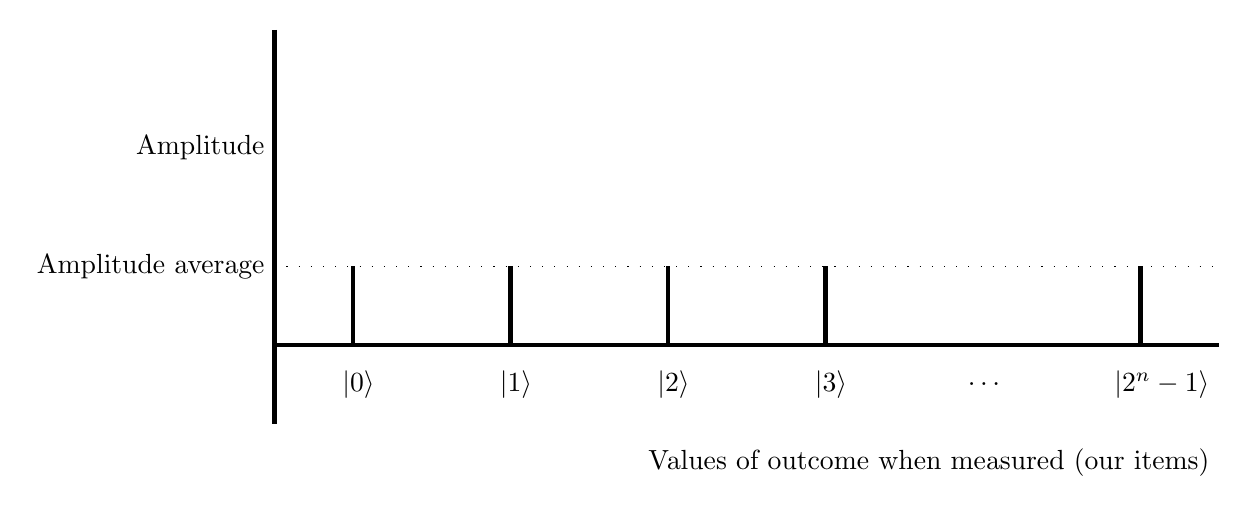
\begin{tikzpicture}
\draw[black, ultra thick] (0,0) -- (12,0);
\draw[black, ultra thick] (0,4) -- (0,-1);

\draw[black, ultra thick] (1,0) -- (1,1);
\draw[black] (1.4,-0.5) node[anchor=east]{$|0\rangle$};

\draw[black, ultra thick] (3,0) -- (3,1);
\draw[black] (3.4,-0.5) node[anchor=east]{$|1\rangle$};

\draw[black, ultra thick] (5,0) -- (5,1);
\draw[black] (5.4,-0.5) node[anchor=east]{$|2\rangle$};

\draw[black, ultra thick] (7,0) -- (7,1);
\draw[black] (7.4,-0.5) node[anchor=east]{$|3\rangle$};


\draw[black] (9.4,-0.5) node[anchor=east]{\dots};


\draw[black, loosely dotted] (0,1) -- (12,1);
\draw[black] (0,1) node[anchor=east]{Amplitude average};

\draw[black, ultra thick] (11,0) -- (11,1);
\draw[black] (12,-0.5) node[anchor=east]{$|2^{n} -1\rangle$};




\draw[black] (0,2.5) node[anchor=east]{Amplitude};
\draw[black] (12,-1.5) node[anchor=east]{Values of outcome when measured (our items)};
\end{tikzpicture}
\caption{Initial superposition of all items} \label{state_pref_graph}
\end{figure}
\end{center}

We represented the numbers in the kets in decimal format, but we refer to them as they would be in binary, this brings little bit of ambiguity because $|0\rangle$ in our diagram can represent the state $|00\rangle$ or $|000\rangle$, but from context it should be clear (in the following parts this will not be discussed, and the reader should be aware). 


\subsection{Applying oracle}
In this part of the algorithm, we point out correct solutions from our database. This can be done by performing a sequence of gates, which switches the amplitude of the correct solution to negative. Remember that we were precisely talking about not absolutely unifying the amplitude and probability in discussion about eq. \ref{one_qubit_}. Performing an oracle operation does not change the probability of measuring the correct result, it only changes the amplitude on the correct result. Oracle will be defined as a function $\mathfrak{O}$, which tells us whether $i$ in the combination \ref{mlti_qubit_state_chapter_2} is a solution or not. More formally, let $\mathfrak{O}:\{0,1\}^n \rightarrow \{0,1\}$, $\mathfrak{O}(\chi)=1$, if $|\chi\rangle$ is a solution, $\mathfrak{O}(\chi)=0$ otherwise. Then the matrix representation has the following pattern:

\begin{equation}
O = 
    \begin{bmatrix}
        -1^{\mathfrak{O}(|0\rangle)} & 0 & 0 & \cdots  & 0 & 0\\ 
        0 & -1^{\mathfrak{O}(|1\rangle)} & 0 & \cdots  & 0 & 0\\
        0 & 0 & -1^{\mathfrak{O}(|2\rangle)} & \cdots  & 0 & 0 \\
        \vdots & \vdots & \vdots & \ddots & \vdots & \vdots \\
        0 & 0 & 0 & \cdots  & -1^{\mathfrak{O}(|n-2\rangle)} & 0 \\
        0 & 0 & 0 & \cdots  & 0 & -1^{\mathfrak{O}(|n-1\rangle)} \\

    \end{bmatrix}.
\end{equation}

We will show that $O$ is unitary. For $O$ to be unitary it would have to mean:

\begin{equation}
    O \cdot \overline{O}^T =I.
\end{equation}
It is simple to see, that there is no imaginary number and transposing diagonal matrix will leave all the elements on the same place. The question now becomes if 

\begin{equation}
    O = O^{-1}.
\end{equation}

This, again, from simple observation is true, because the element on position $o_{j,j}$ can be 1 or -1. If it is 1, then, after multiplying it stays the same; if it is -1, then multiplying changes the value of $o_{j,j}$ to 1, therefore $O = O^{-1}$.

For a simple example, let $|0\rangle$ be the solution. So our diagram then changes as follows. In our diagram, it will be displayed as a visualisation of $|0\rangle$ as magenta instead of black.

\begin{center}
\begin{figure}[h]
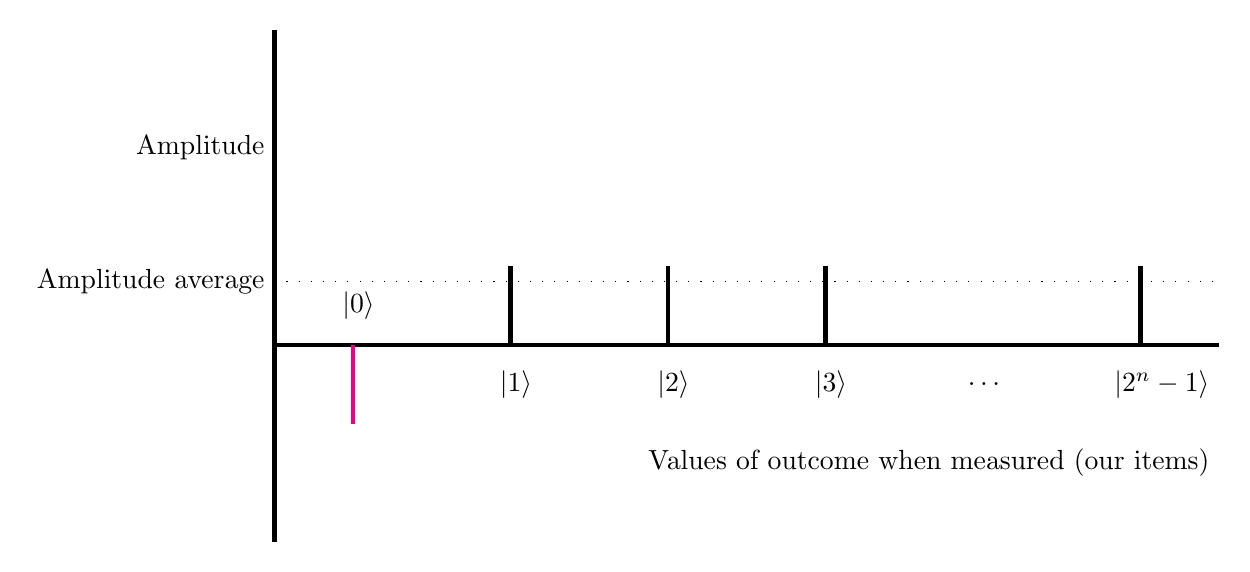
\begin{tikzpicture}
\draw[black, ultra thick] (0,0) -- (12,0);
\draw[black, ultra thick] (0,4) -- (0,-2.5);

\draw[magenta, ultra thick] (1,0) -- (1,-1);
\draw[black] (1.4,0.5) node[anchor=east]{$|0\rangle$};

\draw[black, ultra thick] (3,0) -- (3,1);
\draw[black] (3.4,-0.5) node[anchor=east]{$|1\rangle$};

\draw[black, ultra thick] (5,0) -- (5,1);
\draw[black] (5.4,-0.5) node[anchor=east]{$|2\rangle$};

\draw[black, ultra thick] (7,0) -- (7,1);
\draw[black] (7.4,-0.5) node[anchor=east]{$|3\rangle$};


\draw[black] (9.4,-0.5) node[anchor=east]{\dots};


\draw[black, loosely dotted] (0,0.8) -- (12,0.8);
\draw[black] (0,0.8) node[anchor=east]{Amplitude average};

\draw[black, ultra thick] (11,0) -- (11,1);
\draw[black] (12,-0.5) node[anchor=east]{$|2^{n} -1\rangle$};




\draw[black] (0,2.5) node[anchor=east]{Amplitude};
\draw[black] (12,-1.5) node[anchor=east]{Values of outcome when measured (our items)};
\end{tikzpicture}
\caption{Applying oracle} 
\end{figure}
\end{center}


We also see that the average amplitude has lowered because of the amplitude change of our result to a negative value instead of a positive. 
\newpage
\subsection{Applying diffuser} \label{TeoreticalDiffuser}
Now we rotate about the mean with the selected item, which has a negative amplitude. This results in something called amplitude amplification, where the selected item has a higher probability of being measured. The matrix representation is given by \begin{equation}
    D = 2 |\psi_{INIT} \rangle\langle \psi_{INIT} | - I;     |\psi_{INIT}\rangle = \sum_{i=0}^{2^n-1} \frac{|i\rangle }{\sqrt{2^n}}.
\end{equation}where $\psi_{INIT}$ is state of the quantum register after the state preparation. The diffuser $D$ can be expressed as following matrix:

\begin{equation}
D = 
    \begin{bmatrix}
        \frac{2}{2^n}-1 & \frac{2}{2^n} & \frac{2}{2^n} & \cdots  & \frac{2}{2^n} & \frac{2}{2^n}\\ 
        \frac{2}{2^n} & \frac{2}{2^n}-1 & \frac{2}{2^n} & \cdots  & \frac{2}{2^n} & \frac{2}{2^n}\\
        \frac{2}{2^n} & \frac{2}{2^n} & \frac{2}{2^n}-1 & \cdots  & \frac{2}{2^n} & \frac{2}{2^n} \\
        \vdots & \vdots & \vdots & \ddots & \vdots & \vdots \\
        \frac{2}{2^n} & \frac{2}{2^n} & \frac{2}{2^n} & \cdots  & \frac{2}{2^n}-1 & \frac{2}{2^n} \\
        \frac{2}{2^n} & \frac{2}{2^n} & \frac{2}{2^n} & \cdots  & \frac{2}{2^n} & \frac{2}{2^n} -1 \\

    \end{bmatrix}.
\end{equation}


\begin{center}
\begin{figure}
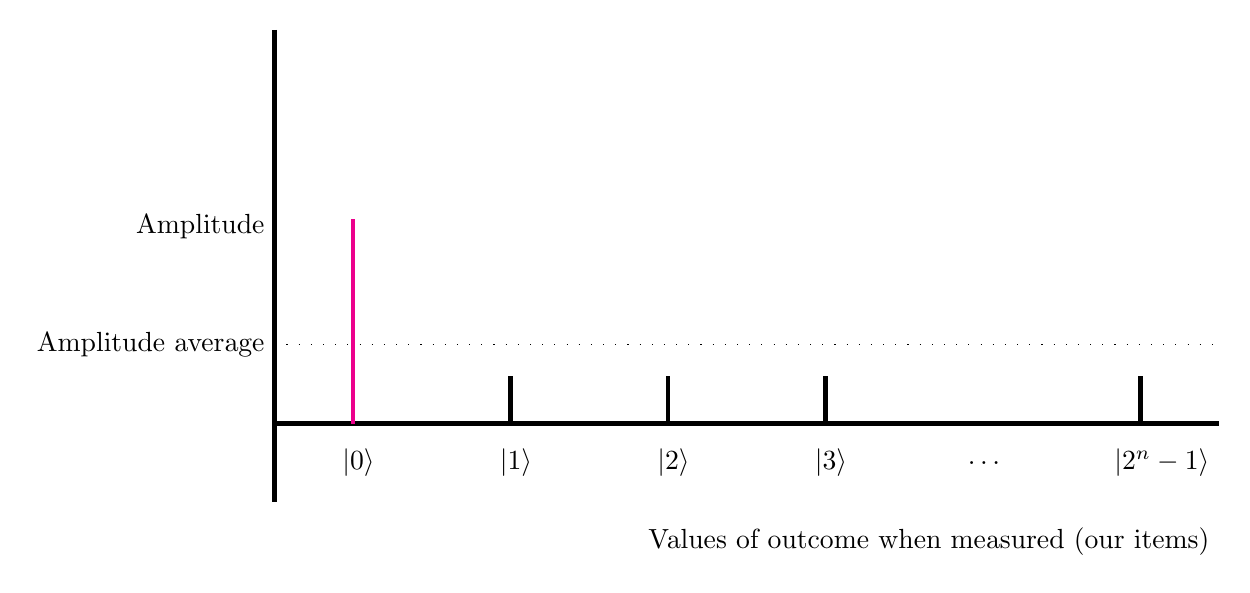
\begin{tikzpicture}
\draw[black, ultra thick] (0,0) -- (12,0);
\draw[black, ultra thick] (0,5) -- (0,-1);

\draw[magenta, ultra thick] (1,0) -- (1,2.6);
\draw[black] (1.4,-0.5) node[anchor=east]{$|0\rangle$};

\draw[black, ultra thick] (3,0) -- (3,0.6);
\draw[black] (3.4,-0.5) node[anchor=east]{$|1\rangle$};

\draw[black, ultra thick] (5,0) -- (5,0.6);
\draw[black] (5.4,-0.5) node[anchor=east]{$|2\rangle$};

\draw[black, ultra thick] (7,0) -- (7,0.6);
\draw[black] (7.4,-0.5) node[anchor=east]{$|3\rangle$};


\draw[black] (9.4,-0.5) node[anchor=east]{\dots};


\draw[black, loosely dotted] (0,1) -- (12,1);
\draw[black] (0,1) node[anchor=east]{Amplitude average};

\draw[black, ultra thick] (11,0) -- (11,0.6);
\draw[black] (12,-0.5) node[anchor=east]{$|2^{n} -1\rangle$};




\draw[black] (0,2.5) node[anchor=east]{Amplitude};
\draw[black] (12,-1.5) node[anchor=east]{Values of outcome when measured (our items)};
\end{tikzpicture}
\caption{Diffuser apply} 
\end{figure}
\end{center}
\newpage
\subsection{Further iterations description}
With the basic concept described, we can perform another repetition of applying the oracle and the diffuser to our quantum register.

Oracle apply:
\begin{center}
\begin{figure}[h]
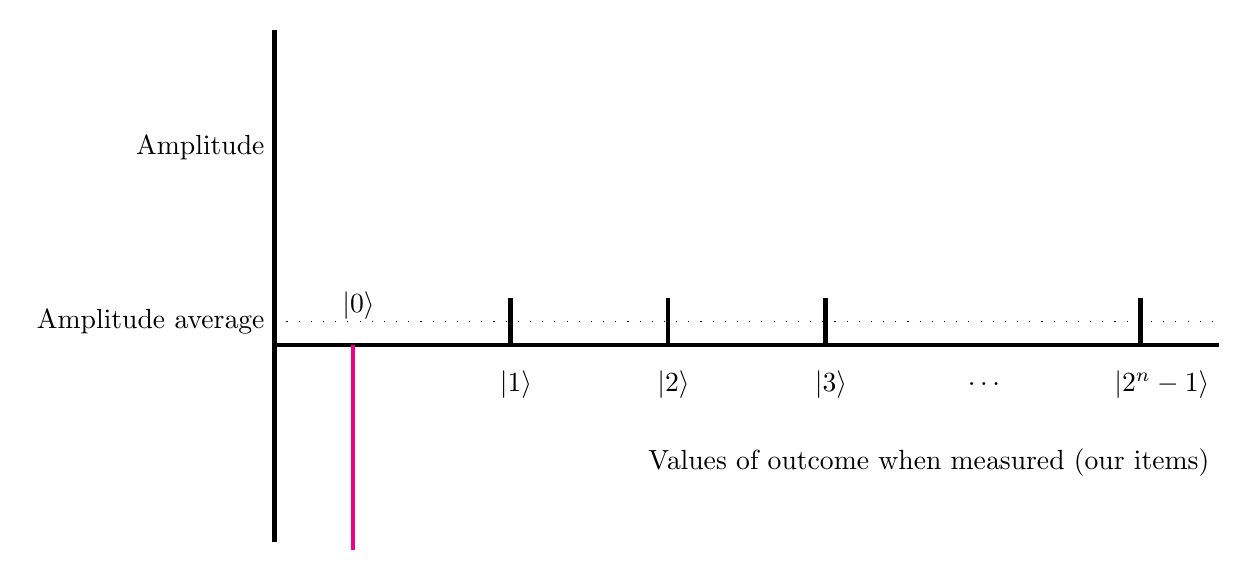
\begin{tikzpicture}
\draw[black, ultra thick] (0,0) -- (12,0);
\draw[black, ultra thick] (0,4) -- (0,-2.5);

\draw[magenta, ultra thick] (1,0) -- (1,-2.6);
\draw[black] (1.4,0.5) node[anchor=east]{$|0\rangle$};

\draw[black, ultra thick] (3,0) -- (3,0.6);
\draw[black] (3.4,-0.5) node[anchor=east]{$|1\rangle$};

\draw[black, ultra thick] (5,0) -- (5,0.6);
\draw[black] (5.4,-0.5) node[anchor=east]{$|2\rangle$};

\draw[black, ultra thick] (7,0) -- (7,0.6);
\draw[black] (7.4,-0.5) node[anchor=east]{$|3\rangle$};


\draw[black] (9.4,-0.5) node[anchor=east]{\dots};


\draw[black, loosely dotted] (0,0.3) -- (12,0.3);
\draw[black] (0,0.3) node[anchor=east]{Amplitude average};

\draw[black, ultra thick] (11,0) -- (11,0.6);
\draw[black] (12,-0.5) node[anchor=east]{$|2^{n} -1\rangle$};




\draw[black] (0,2.5) node[anchor=east]{Amplitude};
\draw[black] (12,-1.5) node[anchor=east]{Values of outcome when measured (our items)};
\end{tikzpicture}
\caption{Second apply of the oracle} 
\end{figure}
\end{center}

Diffuser apply:
\begin{center}
\begin{figure}[h]
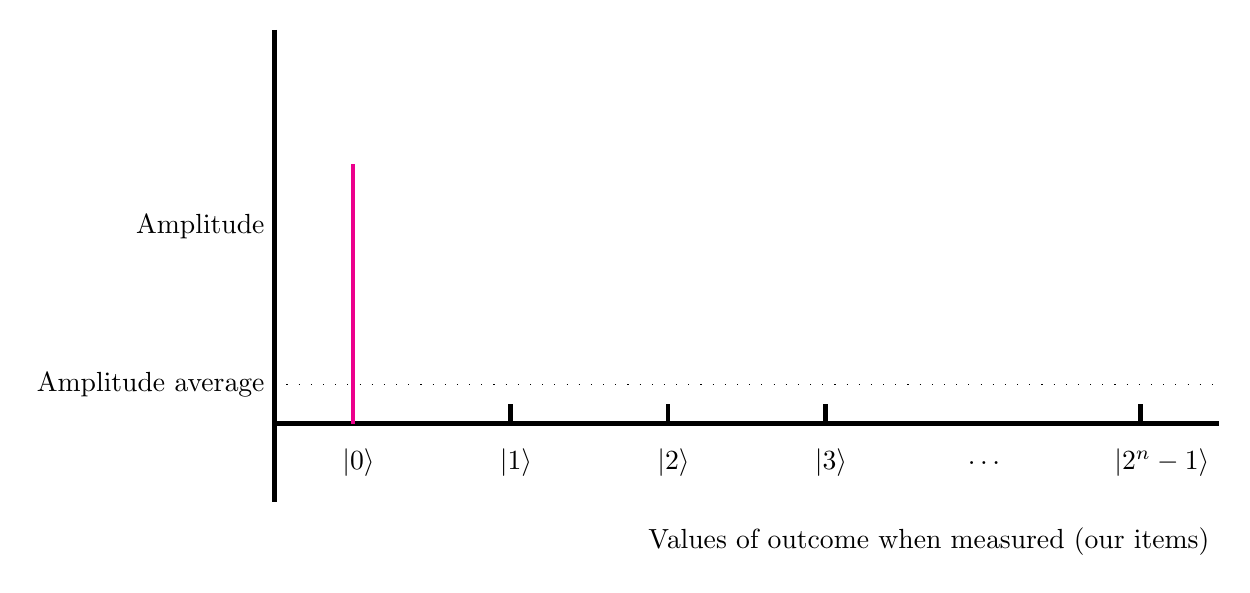
\begin{tikzpicture}
\draw[black, ultra thick] (0,0) -- (12,0);
\draw[black, ultra thick] (0,5) -- (0,-1);

\draw[magenta, ultra thick] (1,0) -- (1,3.3);
\draw[black] (1.4,-0.5) node[anchor=east]{$|0\rangle$};

\draw[black, ultra thick] (3,0) -- (3,0.25);
\draw[black] (3.4,-0.5) node[anchor=east]{$|1\rangle$};

\draw[black, ultra thick] (5,0) -- (5,0.25);
\draw[black] (5.4,-0.5) node[anchor=east]{$|2\rangle$};

\draw[black, ultra thick] (7,0) -- (7,0.25);
\draw[black] (7.4,-0.5) node[anchor=east]{$|3\rangle$};


\draw[black] (9.4,-0.5) node[anchor=east]{\dots};


\draw[black, loosely dotted] (0,0.5) -- (12,0.5);
\draw[black] (0,0.5) node[anchor=east]{Amplitude average};

\draw[black, ultra thick] (11,0) -- (11,0.25);
\draw[black] (12,-0.5) node[anchor=east]{$|2^{n} -1\rangle$};


            

\draw[black] (0,2.5) node[anchor=east]{Amplitude};
\draw[black] (12,-1.5) node[anchor=east]{Values of outcome when measured (our items)};
\end{tikzpicture}
\caption{Second apply of the diffuser}
\end{figure}
\end{center}

We see that the second apply of the oracle and the diffuser had a much smaller impact on our quantum register. All this time we had an amplitude average positive value, performing one more application of the oracle and the diffuser would result in lowering the chance of the solution being measured because the oracle would set the amplitude average to a negative value; thus, the rotation about the mean would have an unwanted effect on our register.

It is a good idea to show the combined matrix of diffuser and oracle, as it shows more in debt how the algorithm works. We will show this for one solution. For demonstrational purpouses, we assume that $|0\rangle$ is the solution, as we have shown in our diagrams.

\begin{equation}
    \iota = DO =
    \begin{bmatrix}
        \frac{2}{2^n}-1 & \frac{2}{2^n} & \frac{2}{2^n} & \cdots  & \frac{2}{2^n} & \frac{2}{2^n}\\ 
        \frac{2}{2^n} & \frac{2}{2^n}-1 & \frac{2}{2^n} & \cdots  & \frac{2}{2^n} & \frac{2}{2^n}\\
        \frac{2}{2^n} & \frac{2}{2^n} & \frac{2}{2^n}-1 & \cdots  & \frac{2}{2^n} & \frac{2}{2^n} \\
        \vdots & \vdots & \vdots & \ddots & \vdots & \vdots \\
        \frac{2}{2^n} & \frac{2}{2^n} & \frac{2}{2^n} & \cdots  & \frac{2}{2^n}-1 & \frac{2}{2^n} \\
        \frac{2}{2^n} & \frac{2}{2^n} & \frac{2}{2^n} & \cdots  & \frac{2}{2^n} & \frac{2}{2^n} -1 \\
    \end{bmatrix}\cdot
    \begin{bmatrix}
        -1 & 0 & 0 & \cdots  & 0 & 0\\ 
        0 & 1 & 0 & \cdots  & 0 & 0\\
        0 & 0 & 1 & \cdots  & 0 & 0 \\
        \vdots & \vdots & \vdots & \ddots & \vdots & \vdots \\
        0 & 0 & 0 & \cdots  & 1 & 0 \\
        0 & 0 & 0 & \cdots  & 0 & 1 \\

    \end{bmatrix}.
\end{equation}

\begin{equation} \label{one_grover_iteration_matrix}
    \iota =
    \begin{bmatrix}
        
        1-\frac{2}{2^n} & \frac{2}{2^n} & \frac{2}{2^n} & \cdots  & \frac{2}{2^n} & \frac{2}{2^n}\\ 
        -\frac{2}{2^n} & \frac{2}{2^n}-1 & \frac{2}{2^n} & \cdots  & \frac{2}{2^n} & \frac{2}{2^n}\\
        -\frac{2}{2^n} & \frac{2}{2^n} & \frac{2}{2^n}-1 & \cdots  & \frac{2}{2^n} & \frac{2}{2^n} \\
        \vdots & \vdots & \vdots & \ddots & \vdots & \vdots \\
        -\frac{2}{2^n} & \frac{2}{2^n} & \frac{2}{2^n} & \cdots  & \frac{2}{2^n}-1 & \frac{2}{2^n} \\
        -\frac{2}{2^n} & \frac{2}{2^n} & \frac{2}{2^n} & \cdots  & \frac{2}{2^n} & \frac{2}{2^n} -1 \\ 
   
    \end{bmatrix}.
\end{equation}

\section{Algorithm analysis and complexity description}

\subsection{Recurrence equations for the algorithm} \label{Recurrence_eq_grover}
Suppose that we have done the first step, the state preparation, and that currently our quantum register is 

\begin{equation}
    |\psi_{INIT}\rangle =  \sum_{i=0}^{2^n-1} \frac{|i\rangle }{\sqrt{N}} =\sum_{i=0}^{2^n-1}\frac{|i\rangle }{\sqrt{2^n}}.
\end{equation}

First we show a system of linear recurrence equations with a parameter as a potential way to derive optimal number of iterations for one solution.

Say we have $\Lambda$, $\Theta$ $\in {\rm I\!R}$, where $\Lambda$ is the amplitude of the correct solution and $\Theta$ is the amplitude of the bad solution. We can continue with the description with eq. \ref{one_grover_iteration_matrix}. We have assumed that $|0\rangle$ is the solution; this means that the first row in the matrix represents an increase or decrease in $\Lambda$. As the algorithm is iterative, we can describe it with a sequence. $\Lambda$ in the $k+1$th step will be equal to

\begin{equation} \label{lambda_increment_first}
    \Lambda_{k+1} = (1-\frac{2}{2^n})\Lambda_k + (2^n -1)\frac{2}{2^n}\Theta_k,
\end{equation}
which can be rewritten as
\begin{equation}
    \Lambda_{k+1}= (1-\frac{2}{2^n})\Lambda_k + (2 - \frac{2}{2^n})\Theta_k.
\end{equation}
Similarly $\Theta$ in the $k+1$th step will be
\begin{equation}
    \Theta_{k+1} = -\frac{2}{2^n}\Lambda_k +(\frac{2}{2^n}-1)\Theta_k +(2^n -2)\frac{2}{2^n}\Theta_k,
\end{equation}
rewriting it as
    \begin{equation}
    \Theta_{k+1} = -\frac{2}{2^n}\Lambda_k +(\frac{2}{2^n}-1 +2 -\frac{4}{2^n})\Theta_k,
    \end{equation}
after simplification,
\begin{equation}
    \Theta_{k+1} = -\frac{2}{2^n}\Lambda_k +(1 -\frac{2}{2^n})\Theta_k.
\end{equation}

Suppose that we have $m$ solutions and $n$ qubits. Then the solution will be slightly different. In eq. \ref{one_grover_iteration_matrix} it would lead to $m$ rows being multiplied by minus one in addition to just one solution. 

\begin{equation} 
    \Lambda_{k+1} = (1-\frac{2}{2^n})\Lambda_k - (m-1)\frac{2}{2^n}\Lambda_k + (2^n - m)\frac{2}{2^n}\Theta_k,
\end{equation}

\begin{equation} 
    \Lambda_{k+1} = (1-\frac{2}{2^n} - \frac{2m}{2^n} +\frac{2}{2^n})\frac{2}{2^n}\Lambda_k + (2^n - m)\frac{2}{2^n}\Theta_k,
\end{equation}

\begin{equation} \label{multi_solution_lambda_last}
    \Lambda_{k+1} = (1 - \frac{2m}{2^n})\Lambda_k + (2^n - m)\frac{2}{2^n}\Theta_k,
\end{equation}

we see that if $m=1$ we get the eq. \ref{lambda_increment_first}. Let us do the same thing for $\Theta$

\begin{equation} 
    \Theta_{k+1} = -\frac{2}{2^n}m\Lambda_k +(\frac{2}{2^n}-1)\Theta_k +(2^n - m -1)\frac{2}{2^n}\Theta_k,
\end{equation}

\begin{equation} 
    \Theta_{k+1} = -\frac{2}{2^n}m\Lambda_k +(\frac{2}{2^n}-1 + 2 - \frac{2m}{2^n} -\frac{2}{2^n})\Theta_k,
\end{equation}

\begin{equation} \label{multi_solution_theta_last}
    \Theta_{k+1} = -\frac{2}{2^n}m\Lambda_k +(1 -\frac{2m}{2^n})\Theta_k,
\end{equation}


We shall discuss eq. \ref{multi_solution_lambda_last} and eq. \ref{multi_solution_theta_last}. $\Lambda_k$ will have the highest value when $\Delta_{k}=\Lambda_{k+1}-\Lambda_k$ reaches the first negative value.
\subsection{Geometrical analysis}

From subsection \ref{Recurrence_eq_grover} we can see that the number of iterations depends on the number of solutions and on the number of qubits used. We will start with one solution and $n$ qubits, we will approach it from one of the perspectives shown in \cite{qc_grover} and \cite{qc_grover_microsoft}.

We begin by constructing a plane $\mathbb{G}$ with two orthogonal states $|\tau\rangle$ and $|\upsilon\rangle$ and our initial state $|\psi_{INIT} \rangle$ and an angle $\frac{\phi}{2}$, which is the angle between $|\psi_{INIT} \rangle$ and $|\upsilon\rangle.$ Let us also define an angle $\zeta$, which is the angle between $|\psi\rangle$ and $|\upsilon\rangle$, after initialization it is same as $\frac{\phi}{2}$.We can express any state in this plane with
\begin{equation} \label{basic_quantum_state_geom}
    |\psi\rangle = \alpha |\tau \rangle  + \beta|\upsilon\rangle.
\end{equation}

Difference between $\alpha$ and $\beta$ from eq. \ref{basic_quantum_state} and from eq. \ref{basic_quantum_state_geom} is that in eq. \ref{basic_quantum_state_geom} $\alpha$, $\beta \in{\rm I\!R}$, while in eq. \ref{basic_quantum_state} $\alpha$, $\beta \in \mathbb{C}$.

With substitution to eq. \ref{basic_quantum_state_geom} we can rewrite it as
\begin{equation}
    |\psi_{INIT}\rangle = sin\Bigl(\frac{\phi}{2}\Bigr)|\tau \rangle  + cos\Bigl(\frac{\phi}{2}\Bigr)|\upsilon\rangle,
\end{equation}

\begin{figure}[h]
\begin{center}
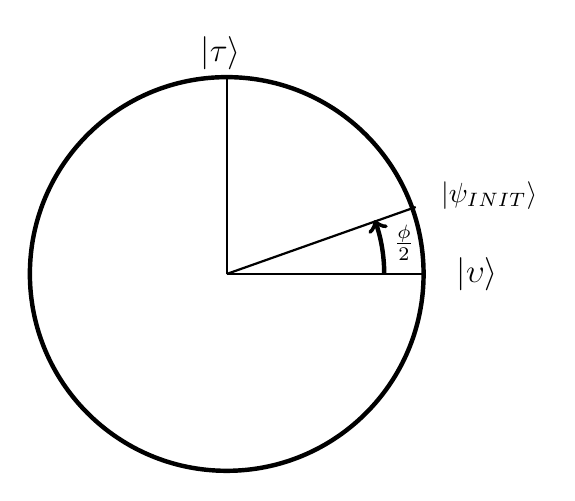
\begin{tikzpicture}
\draw[ultra thick](0,0) circle (2.5);

\draw[black,thick] (0,0) -- (2.5,0);
\draw[black] (0.3,2.8) node[anchor=east,font=\large]{$|\tau\rangle$};

\draw[black, thick] (0,0) -- (0,2.5);
\draw[black] (2.8,0) node[anchor=west,font=\large]{$|\upsilon\rangle$};

\draw[black, thick] (0,0) -- (2.4,0.85);
\draw[black] (2.6,1) node[anchor=west,font=\normalsize]{$|\psi_{INIT}\rangle$};

\draw[ultra thick, ->] (2,0) arc (0:20:2);
\draw[black] (2,0.4) node[anchor=west,font=\normalsize]{$\frac{\phi}{2}$};


\end{tikzpicture}
\caption{Preparation} \label{GA_prep}
\end{center}
\end{figure}

Let's introduce an oracle and its effect on $|\psi_{INIT}\rangle$. Say, we have $|\omega\rangle$ and $|\omega^{\perp}\rangle$, which is orthogonal to $|\omega\rangle$ in $\mathbb{G}$. Let us have $\Hat{\psi}=\Hat{\alpha}|\omega\rangle + \Hat{\beta}|\omega^{\perp}\rangle$. This is satisfied by
\begin{equation}
    |\omega\rangle = sin\Bigl(\Hat{\phi}\Bigr)|\tau \rangle  + cos\Bigl(\Hat{\phi}\Bigr)|\upsilon\rangle
\end{equation}
and
\begin{equation}
    |\omega^{\perp}\rangle = cos\Bigl(\Hat{\phi}\Bigr)|\tau \rangle  -sin\Bigl(\Hat{\phi}\Bigr)|\upsilon\rangle
\end{equation}
This can be shown easily by showing
\begin{equation}
    \langle \omega^{\perp}|\omega\rangle = 0.
\end{equation}
\begin{equation}
     \biggl(cos\Bigl(\Hat{\phi}\Bigr)\langle\tau |  -sin\Bigl(\Hat{\phi}\Bigr)\langle \upsilon|\biggl)\biggl(sin\Bigl(\Hat{\phi}\Bigr)|\tau \rangle  + cos\Bigl(\Hat{\phi}\Bigr)|\upsilon\rangle\biggl),
\end{equation}

\begin{equation}
     cos^2\Bigl(\Hat{\phi}\Bigr)\langle\tau | \upsilon \rangle -sin^2\Bigl(\Hat{\phi}\Bigr)\langle \upsilon|\tau \rangle + sin\Bigl(\Hat{\phi}\Bigr)cos\Bigl(\Hat{\phi}\Bigr)\langle\tau|\tau \rangle  - sin\Bigl(\Hat{\phi}\Bigr)cos\Bigl(\Hat{\phi}\Bigr)\langle\upsilon|\upsilon\rangle,
\end{equation}
$|\upsilon\rangle$ and $|\tau\rangle$ are orthogonal,
\begin{equation}
sin\Bigl(\Hat{\phi}\Bigr)cos\Bigl(\Hat{\phi}\Bigr)\langle\tau|\tau \rangle  - sin\Bigl(\Hat{\phi}\Bigr)cos\Bigl(\Hat{\phi}\Bigr)\langle\upsilon|\upsilon\rangle,
\end{equation}
$\langle\psi|\psi\rangle=1$ for any state $|\psi\rangle$,
\begin{equation}
    sin\Bigl(\Hat{\phi}\Bigr)cos\Bigl(\Hat{\phi}\Bigr)  - sin\Bigl(\Hat{\phi}\Bigr)cos\Bigl(\Hat{\phi}\Bigr) =0.
\end{equation}
Oracle leads to rotation around $|\upsilon\rangle$ in fig. \ref{GA_prep}.


\begin{figure}[ht]
\begin{center}
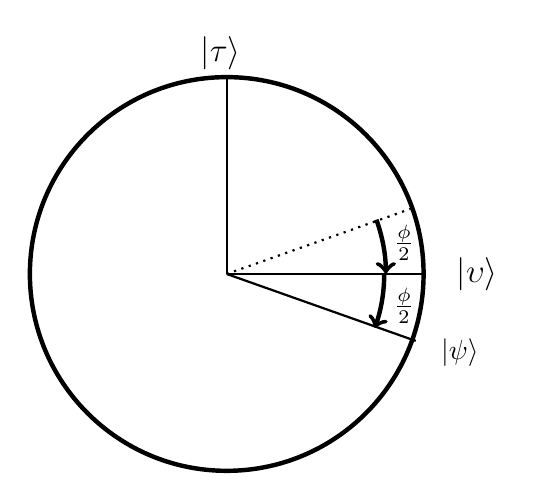
\begin{tikzpicture}
\draw[ultra thick](0,0) circle (2.5);

\draw[black,thick] (0,0) -- (2.5,0);
\draw[black] (0.3,2.8) node[anchor=east,font=\large]{$|\tau\rangle$};

\draw[black, thick] (0,0) -- (0,2.5);
\draw[black] (2.8,0) node[anchor=west,font=\large]{$|\upsilon\rangle$};

\draw[black, thick,dotted] (0,0) -- (2.4,0.85);


\draw[ultra thick, ->] (1.9,0.69) arc (20:0:2);
\draw[black] (2,0.4) node[anchor=west,font=\normalsize]{$\frac{\phi}{2}$};

\draw[ultra thick, ->] (2,0) arc (0:-20:2);
\draw[black] (2,-0.4) node[anchor=west,font=\normalsize]{$\frac{\phi}{2}$};

\draw[black, thick] (0,0) -- (2.4,-0.85);
\draw[black] (2.6,-1) node[anchor=west,font=\normalsize]{$|\psi\rangle$};

\end{tikzpicture}
\caption{Oracle rotation} \label{GA_oracle_geom}
\end{center}
\end{figure}


\begin{equation}
    |\psi\rangle = O|\psi_{INIT}\rangle = -sin\Bigl(\frac{\phi}{2}\Bigr)|\tau \rangle  + cos\Bigl(\frac{\phi}{2}\Bigr)|\upsilon\rangle,
\end{equation}
It is worth pointing out, that the angle $\zeta$ changes to $\frac{-\theta}{2}$, but the functions  have the properties of $sin(-x)=-sin(x)$ and $cos(x)=cos(-x)$.

%From observation we see that $|\psi_{INIT}\rangle\perp O|\psi_{INIT}\rangle$ in $|\omega\rangle$ and $|\omega^{\perp}\rangle$ basis as we defined it as orthogonal.

The iteration ends with the application of the diffuser.  Let us define the diffuser as $D = 2|\omega\rangle\langle\ \omega|-I$, then the diffuser has the following effect.
\begin{equation}
    D\Hat{\psi}=D(\Hat{\alpha}|\omega\rangle + \Hat{\beta}|\omega^{\perp}\rangle),
\end{equation}
after expanding D,
\begin{equation}
    D\Hat{\psi}=(2|\omega\rangle\langle\omega|-I)(\Hat{\alpha}|\omega\rangle + \Hat{\beta}|\omega^{\perp}\rangle),
\end{equation}

\begin{equation}
    D\Hat{\psi}=(2\Hat{\alpha}|\omega\rangle\langle\omega|\omega\rangle-\Hat{\alpha}|\omega\rangle) + 2\Hat{\beta}|\omega\rangle\langle\omega|\omega^{\perp}\rangle - \Hat{\beta}|\omega^{\perp}\rangle,
\end{equation}
$\langle\omega|\omega\rangle=1$ and $\langle\omega|\omega^{\perp}\rangle=0$ leads to
\begin{equation}
    D\Hat{\psi}=\Hat{\alpha}|\omega\rangle - \Hat{\beta}|\omega^{\perp}\rangle.
\end{equation}

In our plane $\mathbb{G}$ this leads to the following reflection, where we choose $\Hat{\phi}=\frac{\phi}{2}$.

\begin{figure}[h]
\begin{center}
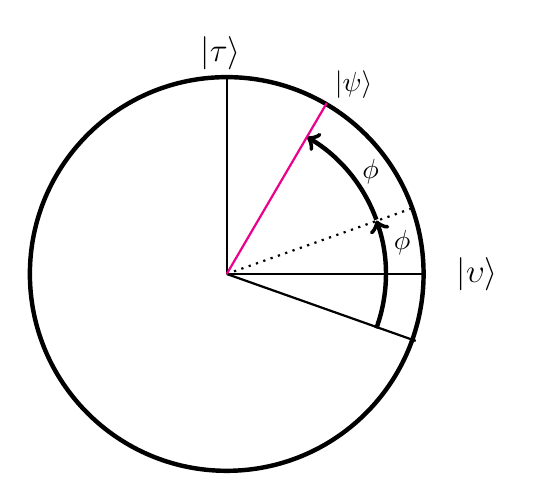
\begin{tikzpicture}
\draw[ultra thick](0,0) circle (2.5);

\draw[black,thick] (0,0) -- (2.5,0);
\draw[black] (0.3,2.8) node[anchor=east,font=\large]{$|\tau\rangle$};

\draw[black, thick] (0,0) -- (0,2.5);
\draw[black] (2.8,0) node[anchor=west,font=\large]{$|\upsilon\rangle$};

\draw[black, thick,dotted] (0,0) -- (2.4,0.85);


\draw[ultra thick, ->] (1.9,-0.69) arc (-20:20:2);
\draw[black] (2,0.4) node[anchor=west,font=\normalsize]{$\phi$};

\draw[ultra thick, ->] (1.9,0.69) arc (20:60:2);
\draw[black] (1.6,1.3) node[anchor=west,font=\normalsize]{$\phi$};

\draw[black, thick] (0,0) -- (2.4,-0.85);

\draw[magenta, thick] (0,0) -- (1.27,2.17);
\draw[black] (1.25,2.4) node[anchor=west,font=\normalsize]{$|\psi\rangle$};

\end{tikzpicture}
\caption{Diffuser reflection} \label{GA_diffuser_geom}
\end{center}
\end{figure}
After applying the oracle the angle stayed the same as we see in fig. \ref{GA_oracle_geom}, the only change was it changed to negative value. The difference was made with the diffuser, since the diffuser had reflection about $|\psi_{INIT}\rangle$, so one iteration $\iota$ of the algorithm increases $\zeta$ by the angle $\phi$ as seen in the figures.

After the iteration, the angle increases, this leads to 
\begin{equation}
    |\psi\rangle = sin\Bigl(\frac{3\phi}{2}\Bigr)|\tau \rangle  + cos\Bigl(\frac{3\phi}{2}\Bigr)|\upsilon\rangle,
\end{equation}
so after $k$ iterations the formula looks like following:
\begin{equation}
        |\psi\rangle = sin\Bigl(\phi k+\frac{\phi}{2}\Bigr)|\tau \rangle  + cos\Bigl(\phi k+\frac{\phi}{2}\Bigr)|\upsilon\rangle,
\end{equation}
which can be rewritten as
\begin{equation}
        |\psi\rangle = sin \Bigl(\phi (k+\frac{1}{2})\Bigr)|\tau \rangle  + cos\Bigl(\phi (k+\frac{1}{2})\Bigr)|\upsilon\rangle,
\end{equation}
so $\zeta = \phi (k+\frac{1}{2}).$

We can view $\tau$ as a solution to the problem and $ \upsilon $ not as a solution. As we are discussing a situation with one solution,
\begin{equation}
    |\psi_{INIT}\rangle=\sqrt{\frac{1}{2^n}}|\tau\rangle+\sqrt{1-\frac{1}{2^n}}|\upsilon\rangle.
\end{equation}
For small angles, we can estimate $\sqrt{\frac{1}{2^n}}=sin(\frac{\phi}{2})\approx\frac{\phi}{2}$.

We want to minimise the probability of measuring $|\upsilon\rangle$, which is given by $cos^2\Bigl(\phi (k+\frac{1}{2})\Bigr)$. This function has its first local minimum in $\frac{\pi}{2}$.

\begin{equation}
    \frac{\pi}{2} = \phi (k+\frac{1}{2}),
\end{equation}
using approximation for $\phi$,
\begin{equation}
    \frac{\pi}{2} = 2\sqrt{\frac{1}{2^n}} (k+\frac{1}{2}),
\end{equation}

\begin{equation}
    \frac{\pi}{2} = 2\sqrt{\frac{1}{2^n}} k+\sqrt{\frac{1}{2^n}},
\end{equation}
\begin{equation}
    \frac{\pi}{2}\sqrt{2^n} = 2k+1,
\end{equation}
\begin{equation}
    k=\frac{\pi}{4}\sqrt{2^n}-\frac{1}{2}.
\end{equation}
With taking $m$ solutions rather than one our approximation for $\frac{\phi}{2}$ would be $\sqrt{\frac{m}{2^n}}=sin(\frac{\phi}{2})\approx\frac{\phi}{2}$, leading to small change in solution.
\begin{equation} \label{optimal_iter}
    k=\frac{\pi}{4}\sqrt\frac{2^n}{m}-\frac{1}{2}.
\end{equation}

We have shown the optimal number of iterations with this geometrical approach.

\chapter{Examples of usage of Grover's algorithm} \label{Practical_ch}

\section{Note on creating an oracle}
To understand how to create a quantum circuit that performs Grover's search, it is important to understand how to create an oracle. It is because the diffuser's matrix always has the same form, see sec. \ref{TeoreticalDiffuser}. Let us describe the pattern on the 3 following circuits.

\subsection{Basic concept}\label{basic_oracle}
We will show the most simple oracle on a circuit made with 2 qubits.
\begin{align}
\Qcircuit @C=1em @R=.7em {
& & & \psi_0 & &  & \psi_1 \\
 &\lstick{\ket{0}} &\qw& \gate{H}& \qw &\ctrl{1} &  \qw &\qw &\\
 &\lstick{\ket{0}} & \gate{X} & \gate{H}&\qw & \gate{X} &  \qw &\qw & \\
}
\end{align}

There, we are going to focus only on the first qubit, as it is the one that we are performing an oracle on.

At $\psi_0$ the first qubit is in state $|+\rangle$ and the second is in state $\psi_1$ is in state $|-\rangle$.
\begin{equation}
|\psi_0\rangle = |+\rangle \otimes |-\rangle = \frac{|0\rangle + |1\rangle}{\sqrt{2}} \otimes \frac{|0\rangle - |1\rangle}{\sqrt{2}} = \frac{(|0\rangle + |1\rangle)(|0\rangle - |1\rangle) }{2}.
\end{equation}
It is important to remember that the tensor product is not comutative.
\begin{equation}
|\psi_0\rangle = \frac{|00\rangle - |01\rangle + |10\rangle - |11\rangle }{2}.
\end{equation}
CNOT swaps the value at the second qubit if the first is $|1\rangle$. After CNOT operation we get $\psi_1$, which has the following form.

\begin{equation}
|\psi_1\rangle = \frac{|00\rangle - |01\rangle + |11\rangle - |10\rangle }{2}=\frac{|00\rangle - |01\rangle -(-|11\rangle) - |10\rangle }{2} = \frac{|0\rangle - |1\rangle}{\sqrt{2}} \otimes \frac{|0\rangle - |1\rangle}{\sqrt{2}}
\end{equation}
We see that the oracle has changed the value of $|1\rangle$, in the Grover's algorithm this means that $|1\rangle$ is the solution.
\subsection{Basic concept with X gate} \label{basic_oracle_x}
This time, we have almost the same circuit as before. The only difference is with a introduction of 2 X gates.

\begin{align}
\Qcircuit @C=1em @R=.7em {
& & & \psi_0 & \psi_1 &  \psi_2 & \psi_3 &  \\
 &\lstick{\ket{0}} & \gate{H} & \qw  &\gate{X} &\ctrl{1} &  \gate{X} &\qw &\\
 &\lstick{\ket{0}} & \gate{X} & \gate{H}& \qw & \gate{X} &  \qw &\qw & \\
}
\end{align}
First part will be same as in example one \ref{basic_oracle}.
\begin{equation}
|\psi_0\rangle = \frac{|00\rangle - |01\rangle + |10\rangle - |11\rangle }{2}.
\end{equation}
Switching the value of the first qubit with the X gate.
\begin{equation}
|\psi_1\rangle = \frac{|10\rangle - |11\rangle + |00\rangle - |01\rangle }{2}.
\end{equation}
Performing CNOT.
\begin{equation}
|\psi_2\rangle = \frac{|11\rangle - |10\rangle + |00\rangle - |01\rangle }{2}.
\end{equation}
Performing the X gate.
\begin{equation}
|\psi_3\rangle = \frac{-(-|01\rangle) - |00\rangle + |10\rangle - |11\rangle }{2} = \frac{-|0\rangle + |1\rangle}{\sqrt{2}} \otimes \frac{|0\rangle - |1\rangle}{\sqrt{2}}.
\end{equation}
This time we selected $|0\rangle$.
\subsection{Basic concept with multicontrol X gate}
This time, we will need 3 qubits.
\begin{align}
\Qcircuit @C=1em @R=.7em {
 && &\psi_0&\psi_1\\
 &\lstick{\ket{0}} &\qw&\gate{H}&\ctrl{2} &  \qw &\\
 &\lstick{\ket{0}} &\qw&\gate{H}&\ctrl{1} &  \qw &\\
 &\lstick{\ket{0}} & \gate{X}&\gate{H}&\gate{X} &  \qw &\\
}
\end{align}

\begin{equation}
|\psi_0\rangle = \frac{|0\rangle + |1\rangle}{\sqrt{2}} \otimes \frac{|0\rangle + |1\rangle}{\sqrt{2}} \otimes \frac{|0\rangle - |1\rangle}{\sqrt{2}}
\end{equation}

\begin{equation}
|\psi_0\rangle =  \frac{|000\rangle - |001\rangle +|010\rangle -|011\rangle +|100\rangle -|101\rangle + |111\rangle - |110\rangle}{2\sqrt{2}}
\end{equation}
After $CNOT_{0,1;2}$.

\begin{equation}
|\psi_1\rangle =  \frac{|00\rangle + |01\rangle + |10\rangle - |11\rangle }{2} \otimes \frac{|0\rangle - |1\rangle}{\sqrt{2}}.
\end{equation}

This time, the selected item was $|11\rangle$. To simply put it, multicontrol acting on $|-\rangle$ will set negative value only for the items (combinations) that perform the swapping on the controlled qubit, this is the reason why we had to switch the first qubit with the X gate in subsec. \ref{basic_oracle_x} to change the value of $|0\rangle$ to negative.

If we had more than one qubit, then selecting $|1\rangle$ on the first qubit would lead to selecting all combinations that have the feature. It would be, for example, $|1001\rangle$, $|1101\rangle$,...

\section{Circuit initialisation and diffuser}
There are multiple ways to create diffusers, we will focus on \cite{qc_grover_ibm}. We will show one that fits our definition and one that does not, but it works with different initialisation. Let us have $n+m+1$ qubits; then the diffuser on the first $n$ qubits that fits the definition will have the following form. It is good to clarify that the X and H gates are performed only on the first $n$ qubits and the second dots represent additional $m$ qubits. It is important to remember that there is a state $|-\rangle$ on the last qubit. 

\newpage
Uncompressed diffuser:
\begin{align}
\Qcircuit @C=1em @R=.7em {
 && &&&&&\\
&\qw & \gate{H} &\gate{X} &\ctrl{6} &\gate{X} &\gate{H} &\qw & \qw & \\
&\qw &\gate{H} &\gate{X} &\ctrl{5} &\gate{X} &\gate{H} & \qw & \qw & \\
&\qw &\gate{H} &\gate{X} &\ctrl{4} &\gate{X} &\gate{H} & \qw & \qw & \\
& &\vdots &\vdots &\vdots &\vdots &\vdots &\\
&& &&&&&\\
 &\qw &\gate{H} &\gate{X} &\ctrl{2} &\gate{X} &\gate{H} &\qw & \qw & \\
 & &\vdots &\vdots &\vdots &\vdots &\vdots &\\
 &\qw & \qw & \qw & \gate{X} &\qw & \qw &\qw &  \\
}
\end{align}
Compressed diffuser:
\begin{align}
\Qcircuit @C=1em @R=.7em {
 && &&&&&\\
&\qw & \gate{H} &\ctrl{6}  &\gate{H} &\qw & \qw & \\
&\qw &\gate{H} &\ctrl{5}  &\gate{H} & \qw & \qw & \\
&\qw &\gate{H}  &\ctrl{4}  &\gate{H} & \qw & \qw & \\
& &\vdots &\vdots &\vdots &\\
&& &&&&&\\
 &\qw &\gate{H}  &\ctrl{2} &\gate{H} &\qw & \qw & \\
 & &\vdots &\vdots &\vdots &\\
 &\qw & \qw  & \gate{X} &\qw  &\qw  &\qw \\
}
\end{align}
Initialisation part for compressed diffuser:

\begin{align}
\Qcircuit @C=1em @R=.7em {
 && &&&&&\\
 &\lstick{\ket{0}} &\gate{X}&\gate{H}\\
 &\lstick{\ket{0}} &\gate{X}&\gate{H}\\
 &\lstick{\ket{0}} &\gate{X}&\gate{H}\\
 & &\vdots &\vdots &\\
  && &&&&&\\
 &\lstick{\ket{0}} &\gate{X}&\gate{H}\\
 & &\vdots &\vdots &\\
 && &&&&&\\
 &\lstick{\ket{0}} & \gate{X}&\gate{H}&\\
}
\end{align}

\section{Small Sudoku}

We will start with a small example. The task is taken from \cite{qc_grover_ibm}. The problem is the following; find the combinations that fit into the following clauses. The first clause is $v_0 \neq v_1 $, the second is $v_0 \neq v_2 $, the third is $v_1 \neq v_3 $ and the last is $v_2 \neq v_3 $, where $v_0, v_1, v_2, v_3 \in \{ 0,1 \}$.

\begin{figure}[h!]
\begin{center}
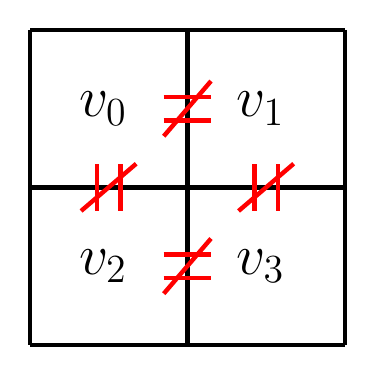
\begin{tikzpicture}


\draw[black, ultra thick] (0,0) -- (4,0);
\draw[black, ultra thick] (0,4) -- (0,0);
\draw[black, ultra thick] (4,4) -- (0,4);
\draw[black, ultra thick] (4,4) -- (4,0);


\draw[black, ultra thick] (0,2) -- (4,2);
\draw[black, ultra thick] (2,0) -- (2,4);

\draw[black] (0.5,3) node[anchor=west,font=\huge]{$v_0$};
\draw[black] (2.5,3) node[anchor=west,font=\huge]{$v_1$};
\draw[black] (0.5,1) node[anchor=west,font=\huge]{$v_2$};
\draw[black] (2.5,1) node[anchor=west,font=\huge]{$v_3$};

\draw[red, ultra thick] (1.7,0.85) -- (2.3,0.85);
\draw[red, ultra thick] (1.7,1.15) -- (2.3,1.15);
\draw[red, ultra thick] (1.7,0.65) -- (2.3,1.35);


\draw[red, ultra thick] (1.7,2.85) -- (2.3,2.85);
\draw[red, ultra thick] (1.7,3.15) -- (2.3,3.15);
\draw[red, ultra thick] (1.7,2.65) -- (2.3,3.35);

\draw[red, ultra thick] (2.85,1.7) -- (2.85,2.3);
\draw[red, ultra thick] (3.15,1.7) -- (3.15,2.3);
\draw[red, ultra thick] (2.65,1.7) -- (3.35,2.3);

\draw[red, ultra thick] (0.85,1.7) -- (0.85,2.3);
\draw[red, ultra thick] (1.15,1.7) -- (1.15,2.3);
\draw[red, ultra thick] (0.65,1.7) -- (1.35,2.3);


\end{tikzpicture}
\caption{Task visualisation} \label{small_sudoku_vis}
\end{center}
\end{figure}






From the observation of the assign, we are able to construct the following equations. Note that the following functions are going to be boolean.
\begin{equation} \label{1st_condition}
    (v_0 \cdot \overline{v_1})+(\overline{v_0} \cdot v_1) = 1
\end{equation}

\begin{equation} \label{2nd_condition}
    (v_0 \cdot \overline{v_2})+(\overline{v_0} \cdot v_2) = 1
\end{equation}

\begin{equation} \label{3rd_condition}
    (v_2 \cdot \overline{v_3})+(\overline{v_3} \cdot v_2) = 1
\end{equation}
We won't cover simple solution in \cite{qc_grover_ibm}, instead, we will focus on smaller solutions, that can run on currently available quantum computers. 

\subsection{Solution with 6 qubits} \label{Solution_with_6_qubits}

The first solution requires 6 qubits, which is a large improvement over the original 9 presented by IBM; the trick is to compact the oracle from 9 to 6 qubits. We will use the following picture to show states during the run of the algorithm. This solution was proposed by the supervisor, Jiří Tomčala, Ph.D.

\begin{align}
\Qcircuit @C=1em @R=.7em {
 &\psi_0& &&&  &&&&&&\psi_1\\
&\qw &\ctrl{4} &  \qw & \ctrl{2} &\qw&\qw&\qw&\ctrl{2}&\qw&\ctrl{4}\qw&\qw&\\
&\qw&\qw & \ctrl{3}\qw &  \qw&\ctrl{2} &\qw&\ctrl{2} &\qw&\ctrl{3}&\qw&\qw&\\
  &\qw&  \qw &  \qw &\gate{X}& \qw &\ctrl{3}&\qw&\gate{X}  &\qw&\qw&\qw&\\
 &\qw&    \qw &  \qw &\qw &\gate{X}&\ctrl{2} &\gate{X}&\qw&\qw&\qw&\qw&\\
 &\qw&\gate{X} &\gate{X} &  \qw &\qw &\ctrl{1} &\qw  &\qw &\gate{X}&\gate{X}&\qw&\\
 &\qw &  \qw &\qw &\qw &\qw &\gate{X} &\qw  &\qw &\qw &\qw&\qw&\\
}
\end{align}
The trick there is we use qubits both for storing value of our result as well as for implementing clauses. The first two CNOTs implement simple functions so that the first and second qubits cannot have the same value. As we pointed out before, the qubit has to be $|1\rangle$ to transfer the negative phase. The third CNOT can be interpreted as the first qubit being not equal to the third. The same goes for the second qubit, where CNOT implements XOR between the second and the fourth qubit. CNOTs after CCCNOT implement some sort of cleaning, so that oracle performs only phase rotation and nothing more. 

To derive states during the run of the algorithm, we will use an uncompressed diffuser, we will observe only states on the first four qubits, as the vector of all 6 qubits would have length of 64.

\begin{align}
\Qcircuit @C=1em @R=.7em {
&\psi_1&\psi_2&\psi_3&\psi_4&\psi_5&\psi_6&&\\
&\qw & \gate{H} &\gate{X} &\ctrl{5} &\gate{X} &\gate{H} &\qw & \qw & \\
&\qw &\gate{H} &\gate{X} &\ctrl{4} &\gate{X} &\gate{H} & \qw & \qw & \\
&\qw &\gate{H} &\gate{X} &\ctrl{3} &\gate{X} &\gate{H} & \qw & \qw & \\
&\qw &\gate{H} &\gate{X} &\ctrl{2} &\gate{X} &\gate{H} &\qw & \qw & \\
&\qw&\qw&\qw&\qw&\qw&\qw&\qw&\qw\\
 &\qw & \qw & \qw & \gate{X} &\qw & \qw &\qw &\qw \\
}
\end{align}
Let $\mathcal{T}=\{1001,0110\} $ and $\mathcal{F}=\{0,1\}^4 \setminus \mathcal{T}$

\begin{equation}
    |\psi_0\rangle =  \sum_{i\in \{0,1\}^4}^{} \frac{|i\rangle }{4}.
\end{equation}

\begin{equation}
    |\psi_1\rangle =  \sum_{i\in \mathcal{F}}^{} \frac{|i\rangle }{4} -\sum_{i\in \mathcal{T}}^{} \frac{|i\rangle }{4}.
\end{equation}

\begin{equation}
    |\psi_2\rangle =  \frac{3}{4}|0000\rangle+\frac{1}{4}|0011\rangle+\frac{1}{4}|0101\rangle-\frac{1}{4}|0110\rangle-\frac{1}{4}|1001\rangle+\frac{1}{4}|1010\rangle+\frac{1}{4}|1100\rangle-\frac{1}{4}|1111\rangle.
\end{equation}

\begin{equation}
    |\psi_3\rangle = \frac{1}{4}|0000\rangle-\frac{1}{4}|0011\rangle-\frac{1}{4}|0101\rangle+\frac{1}{4}|0110\rangle+\frac{1}{4}|1001\rangle-\frac{1}{4}|1010\rangle-\frac{1}{4}|1100\rangle-\frac{3}{4}|1111\rangle.
\end{equation}

\begin{equation}
    |\psi_4\rangle = \frac{1}{4}|0000\rangle-\frac{1}{4}|0011\rangle-\frac{1}{4}|0101\rangle+\frac{1}{4}|0110\rangle+\frac{1}{4}|1001\rangle-\frac{1}{4}|1010\rangle-\frac{1}{4}|1100\rangle+\frac{3}{4}|1111\rangle.
\end{equation}

\begin{equation}
    |\psi_5\rangle = \frac{3}{4}|0000\rangle-\frac{1}{4}|0011\rangle-\frac{1}{4}|0101\rangle+\frac{1}{4}|0110\rangle+\frac{1}{4}|1001\rangle-\frac{1}{4}|1010\rangle-\frac{1}{4}|1100\rangle+\frac{1}{4}|1111\rangle.
\end{equation}

\begin{equation}
    |\psi_6\rangle =  \sum_{i\in \mathcal{F}}^{} \frac{|i\rangle }{8} -\sum_{i\in \mathcal{T}}^{} \frac{5|i\rangle }{8}.
\end{equation}

We can check the results with our recurrence eqs. \ref{multi_solution_lambda_last} and \ref{multi_solution_theta_last}. Let $\Theta_0 = \frac{1}{4}$, $\Lambda_0 = \frac{1}{4}$, $m = 2$, and $n = 4$.

\begin{equation}
    \Lambda_1 = (1-\frac{2\cdot2}{16})\frac{1}{4} + (16-2)\frac{2}{16}\frac{1}{4}=\frac{12}{64}+\frac{28}{64} = \frac{40}{64} = \frac{5}{8}.
\end{equation}

\begin{equation}
    \Theta_1 = -\frac{2}{16}\cdot2\cdot\frac{1}{4} + (1-\frac{2\cdot 2}{16})\frac{1}{4} = \frac{-4}{64}+\frac{12}{64} = \frac{8}{64} = \frac{1}{8}.
\end{equation}
This is exactly the result of simulating our algorithm. We ran algorithm on IBM's device Ibm\_nairobi with following results.

\begin{figure}[H]
\centering
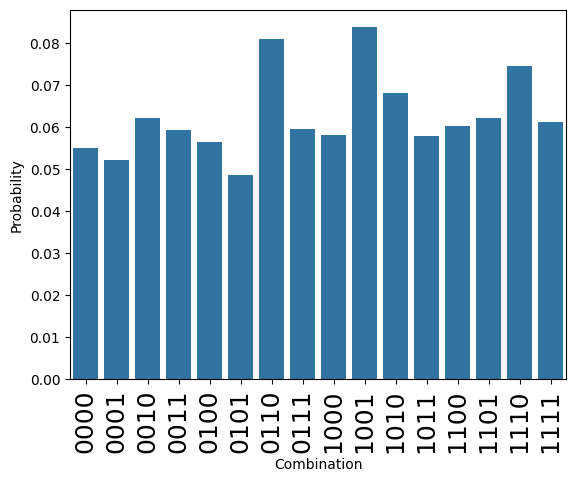
\includegraphics[width=10cm]{Figures/bc0_0.png}
\caption{Results from the QC}
\label{Smallb00}
\end{figure}

Result from simulator:
\begin{figure}[H]
\centering
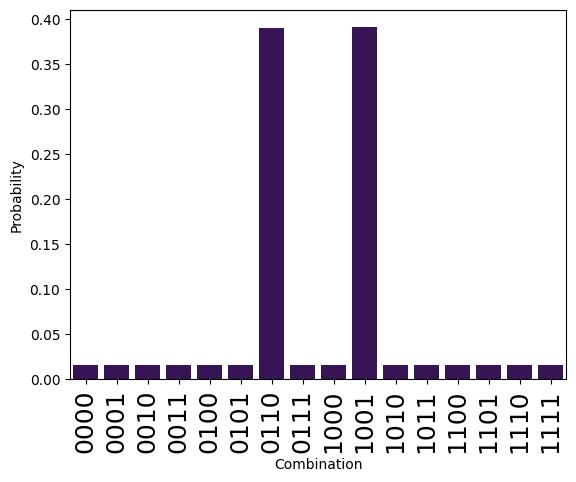
\includegraphics[width=10cm]{Figures/sim0.png}
\caption{Results from the simulator}
\label{sim0}
\end{figure}


We see that even with that small circuit there is a lot of noise, in fig. \ref{Smallb00} the most two observed results are the correct solution to the given problem, but it is easy to see that many other incorrect solutions are observed more, than theoretical computations predicted. The simulation results are comparable to the theoretical values.

\subsection{Solution with 5 qubits}

Now, we are going to focus on equations \ref{1st_condition}, \ref{2nd_condition} and \ref{3rd_condition}, which must be true at the same time, leading to the following expression.
\begin{equation}
    \Bigl( \big(v_0 \cdot \overline{v_1})+(\overline{v_0} \cdot v_1) \Bigl) \cdot \Bigl( (v_0 \cdot \overline{v_2})+(\overline{v_0} \cdot v_2) \Bigl) \cdot \Bigl( (v_2 \cdot \overline{v_3})+(\overline{v_2} \cdot v_3) \Bigl) = 1.
\end{equation}
After distribution,

\begin{equation}
    \Bigl( \big(v_0 \cdot \overline{v_1})+(\overline{v_0} \cdot v_1) \Bigl) \cdot \Bigl( (v_0 \cdot \overline{v_2})+(\overline{v_0} \cdot v_2) \Bigl) \cdot  (v_2 \cdot \overline{v_3})+\Bigl( \big(v_0 \cdot \overline{v_1})+(\overline{v_0} \cdot v_1) \Bigl) \cdot \Bigl( (v_0 \cdot \overline{v_2})+(\overline{v_0} \cdot v_2) \Bigl)(\overline{v_2} \cdot v_3)  = 1.
\end{equation}
Further after second distribution,

\begin{equation}
    \begin{multlined}
        \Bigl( \big(v_0 \cdot \overline{v_1})+(\overline{v_0} \cdot v_1) \Bigl) \cdot \Bigl( (v_0 \cdot \overline{v_2})+(\overline{v_0} \cdot v_2) \Bigl) \cdot  (v_2 \cdot \overline{v_3})+ 
        \\
        \Bigl( \big(v_0 \cdot \overline{v_1})+(\overline{v_0} \cdot v_1) \Bigl) \cdot ( (v_0 \cdot \overline{v_2}) \cdot (\overline{v_2} \cdot v_3) + 
        \\
        \Bigl( \big(v_0 \cdot \overline{v_1})+(\overline{v_0} \cdot v_1) \Bigl) \cdot (\overline{v_0} \cdot v_2) \cdot (\overline{v_2} \cdot v_3) = 1.
        \end{multlined}
\end{equation}  
Sice $A\overline{A}=0$,

\begin{equation}
    \begin{multlined}
        \Bigl( \big(v_0 \cdot \overline{v_1})+(\overline{v_0} \cdot v_1) \Bigl) \cdot \Bigl( (v_0 \cdot \overline{v_2})+(\overline{v_0} \cdot v_2) \Bigl) \cdot  (v_2 \cdot \overline{v_3})+ 
        \\
        \Bigl( \big(v_0 \cdot \overline{v_1})+(\overline{v_0} \cdot v_1) \Bigl) \cdot ( (v_0 \cdot \overline{v_2}) \cdot (\overline{v_2} \cdot v_3) = 1.
        \end{multlined}
\end{equation}
$AA=A$,
\begin{equation}
    \begin{multlined}
        \Bigl( \big(v_0 \cdot \overline{v_1})+(\overline{v_0} \cdot v_1) \Bigl) \cdot \Bigl( (v_0 \cdot \overline{v_2})+(\overline{v_0} \cdot v_2) \Bigl) \cdot  (v_2 \cdot \overline{v_3})+ 
        \\
        \Bigl( \big(v_0 \cdot \overline{v_1})+(\overline{v_0} \cdot v_1) \Bigl) \cdot  (v_0 \cdot \overline{v_2} \cdot v_3) = 1.
        \end{multlined}
\end{equation}
After another distribution.

\begin{equation}
    \begin{multlined}
        \Bigl( \big(v_0 \cdot \overline{v_1})+(\overline{v_0} \cdot v_1) \Bigl) \cdot \Bigl( (v_0 \cdot \overline{v_2})+(\overline{v_0} \cdot v_2) \Bigl) \cdot  (v_2 \cdot \overline{v_3})+ 
        \\
        ( v_0 \cdot \overline{v_1})(v_0 \cdot \overline{v_2} \cdot v_3) + (\overline{v_0} \cdot v_1)(v_0 \cdot \overline{v_2} \cdot v_3) = 1.
        \end{multlined}
\end{equation}
$A\overline{A}=0$ and $AA=A$
\begin{equation}
    \begin{multlined}
        \Bigl( \big(v_0 \cdot \overline{v_1})+(\overline{v_0} \cdot v_1) \Bigl) \cdot \Bigl( (v_0 \cdot \overline{v_2})+(\overline{v_0} \cdot v_2) \Bigl) \cdot  (v_2 \cdot \overline{v_3})+ v_0 \cdot \overline{v_1} \cdot \overline{v_2} \cdot v_3 =1
        \end{multlined}
\end{equation}
Let us apply same steps onto the first part of the equation aswell. 

\begin{equation}
    \begin{multlined}
        \Bigl( \big(v_0 \cdot \overline{v_1})+(\overline{v_0} \cdot v_1) \Bigl) \cdot \Bigl((v_0 \cdot \overline{v_2})(v_2 \cdot \overline{v_3})+(\overline{v_0} \cdot v_2)(v_2 \cdot \overline{v_3})\Bigl) +
        \\
        v_0 \cdot \overline{v_1} \cdot \overline{v_2} \cdot v_3 =1
        \end{multlined}
\end{equation}
Apply identities,
\begin{equation}
    \begin{multlined}
        \Bigl( \big(v_0 \cdot \overline{v_1})+(\overline{v_0} \cdot v_1) \Bigl) \cdot \Bigl( (\overline{v_0} \cdot v_2 \cdot \overline{v_3}\Bigl) +
        v_0 \cdot \overline{v_1} \cdot \overline{v_2} \cdot v_3 =1.
        \end{multlined}
\end{equation}
Applying last distribution,

\begin{equation}
    \begin{multlined}    
        v_0 \cdot \overline{v_1} \cdot\overline{v_0} \cdot v_2 \cdot \overline{v_3} + \overline{v_0} \cdot v_1 \cdot \overline{v_0} \cdot v_2 \cdot  \overline{v_3}+
        v_0 \cdot \overline{v_1} \cdot \overline{v_2} \cdot v_3 =1.
        \end{multlined}
\end{equation}
$A\overline{A}=0$ gives
\begin{equation}
    \begin{multlined}    
       \overline{v_0} \cdot v_1 \cdot v_2 \cdot \overline{v_3}+
        v_0 \cdot \overline{v_1} \cdot \overline{v_2} \cdot v_3 =1.
        \end{multlined}
\end{equation}

This means that we have 2 representations of the same function, we can give a quantum computer to compute. We can also see that the term at the end is shorter and uses fewer gates. The down side of this solution is in CCCCNOT gates, in the original solution there was only one, there are three of them. Such a gate is decomposed into multiple CNOTs and other gates. This leads to the conclusion that this may be more compact, but it will run longer on a quantum computer, thus, more incorrect measurements will be observed.
Oracle:
\begin{align}
\Qcircuit @C=1em @R=.7em {
&\psi_0 & & &\psi_1&&&\psi_2&&\\
&\qw  &\gate{X} &\ctrl{4} &\gate{X}&\qw &\ctrl{4} &\qw  &\qw & \qw & \\
&\qw  & \qw &\ctrl{3} &\qw&\gate{X} &\ctrl{3} &\gate{X}  & \qw & \qw & \\
&\qw  &\qw &\ctrl{2} &\qw&\gate{X} &\ctrl{2} &\gate{X}  & \qw & \qw & \\
&\qw  &\gate{X} &\ctrl{1} &\gate{X}&\qw &\ctrl{1} &\qw  &\qw & \qw & \\
 &\qw & \qw & \gate{X} &\qw & \qw & \gate{X} & \qw & \qw & \qw \\
}
\end{align}
Diffuser:
\begin{align}
\Qcircuit @C=1em @R=.7em {
&\psi_2&\psi_3&\psi_4&\psi_5&\psi_6&\psi_7&&\\
&\qw & \gate{H} &\gate{X} &\ctrl{4} &\gate{X} &\gate{H} &\qw & \qw & \\
&\qw &\gate{H} &\gate{X} &\ctrl{3} &\gate{X} &\gate{H} & \qw & \qw & \\
&\qw &\gate{H} &\gate{X} &\ctrl{2} &\gate{X} &\gate{H} & \qw & \qw & \\
&\qw &\gate{H} &\gate{X} &\ctrl{1} &\gate{X} &\gate{H} &\qw & \qw & \\
 &\qw & \qw & \qw & \gate{X} &\qw & \qw &\qw &\qw \\
}
\end{align}

\begin{equation}
    |\psi_0\rangle =  \sum_{i\in \{0,1\}^4}^{} \frac{|i\rangle }{4}.
\end{equation}

\begin{equation} \label{psi1_small}
    |\psi_1\rangle =  \sum_{i\in \{0,1\}^4\setminus 0110}^{} \frac{|i\rangle }{4} -\frac{|0110\rangle }{4}.
\end{equation}

\begin{equation}
    |\psi_2\rangle =  \sum_{i\in \mathcal{F}}^{} \frac{|i\rangle }{4} -\sum_{i\in \mathcal{T}}^{} \frac{|i\rangle }{4}.
\end{equation}

\begin{equation}
    |\psi_3\rangle =  \frac{3}{4}|0000\rangle+\frac{1}{4}|0011\rangle+\frac{1}{4}|0101\rangle-\frac{1}{4}|0110\rangle-\frac{1}{4}|1001\rangle+\frac{1}{4}|1010\rangle+\frac{1}{4}|1100\rangle-\frac{1}{4}|1111\rangle.
\end{equation}

\begin{equation}
    |\psi_4\rangle = \frac{1}{4}|0000\rangle-\frac{1}{4}|0011\rangle-\frac{1}{4}|0101\rangle+\frac{1}{4}|0110\rangle+\frac{1}{4}|1001\rangle-\frac{1}{4}|1010\rangle-\frac{1}{4}|1100\rangle-\frac{3}{4}|1111\rangle.
\end{equation}

\begin{equation}
    |\psi_5\rangle = \frac{1}{4}|0000\rangle-\frac{1}{4}|0011\rangle-\frac{1}{4}|0101\rangle+\frac{1}{4}|0110\rangle+\frac{1}{4}|1001\rangle-\frac{1}{4}|1010\rangle-\frac{1}{4}|1100\rangle+\frac{3}{4}|1111\rangle.
\end{equation}

\begin{equation}
    |\psi_6\rangle = \frac{3}{4}|0000\rangle-\frac{1}{4}|0011\rangle-\frac{1}{4}|0101\rangle+\frac{1}{4}|0110\rangle+\frac{1}{4}|1001\rangle-\frac{1}{4}|1010\rangle-\frac{1}{4}|1100\rangle+\frac{1}{4}|1111\rangle.
\end{equation}

\begin{equation}
    |\psi_7\rangle =  \sum_{i\in \mathcal{F}}^{} \frac{|i\rangle }{8} -\sum_{i\in \mathcal{T}}^{} \frac{5|i\rangle }{8}.
\end{equation}

After eq. \ref{psi1_small} the algorithm has the same states as \ref{Solution_with_6_qubits}, but it is not surprising as we only made a different oracle and described it in two steps instead of one.

This time we used IBM's Ibm\_nairobi and got the following results.

\begin{figure}[h]
\centering
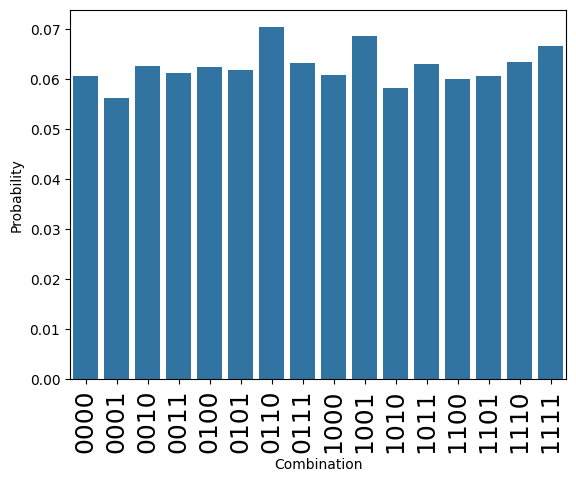
\includegraphics[width=10cm]{Figures/bc1_0.png}
\caption{Results from the QC}
\label{Smallb10}
\end{figure}
Result from simulator:
\begin{figure}[H]
\centering
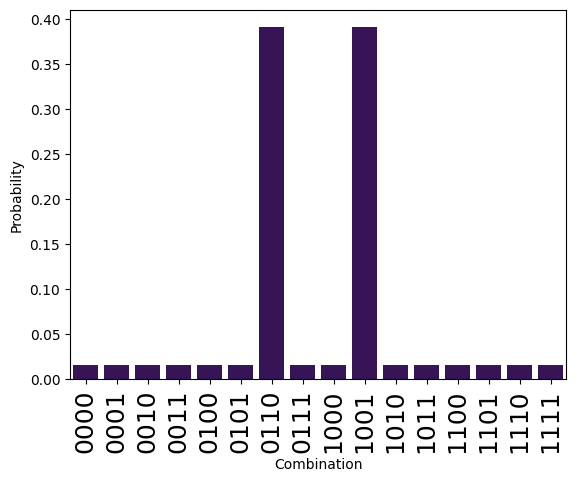
\includegraphics[width=10cm]{Figures/sim1.png}
\caption{Results from the simulator}
\label{sim1}
\end{figure}

We see a similar trend as before, where we have a good result in fig. \ref{Smallb10}, but it is incomparable with \ref{sim1}, where we see that the counts are close to theoretical values. Compared to fig. \ref{Smallb00} we have worse results, as incorrect combinations are measured more, but still the two most measured combinations are solution to the given problem.
\section{Large Sudoku}

We are given a 3x3 grid, in each tile, there can be either 0 or 1. In each row and in each column the sum must be 2.

\begin{figure}[h!]
\begin{center}
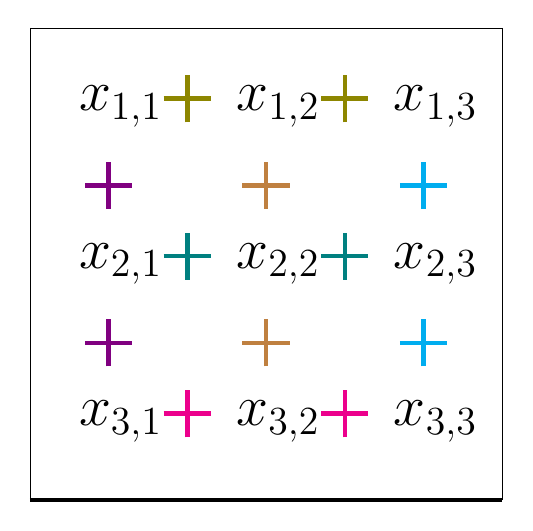
\begin{tikzpicture}


\draw[black, ultra thick] (0,0) -- (6,0);
\draw[black, ultra thin] (0,6) -- (0,0);
\draw[black,ultra  thin] (6,6) -- (0,6);
\draw[black,ultra  thin] (6,6) -- (6,0);

%\draw[black,ultra  thin] (0,2) -- (6,2);
%\draw[black,ultra  thin] (0,4) -- (6,4);

%\draw[black,ultra  thin] (2,0) -- (2,6);
%\draw[black,ultra  thin] (4,0) -- (4,6);

\draw[black] (0.5,1) node[anchor=west,font=\huge]{$x_{3,1}$};
\draw[black] (2.5,1) node[anchor=west,font=\huge]{$x_{3,2}$};
\draw[black] (4.5,1) node[anchor=west,font=\huge]{$x_{3,3}$};

\draw[black] (0.5,3) node[anchor=west,font=\huge]{$x_{2,1}$};
\draw[black] (2.5,3) node[anchor=west,font=\huge]{$x_{2,2}$};
\draw[black] (4.5,3) node[anchor=west,font=\huge]{$x_{2,3}$};

\draw[black] (0.5,5) node[anchor=west,font=\huge]{$x_{1,1}$};
\draw[black] (2.5,5) node[anchor=west,font=\huge]{$x_{1,2}$};
\draw[black] (4.5,5) node[anchor=west,font=\huge]{$x_{1,3}$};

\draw[violet, ultra thick] (0.7,2) -- (1.3,2);
\draw[violet, ultra thick] (1,1.7) -- (1,2.3);

\draw[violet, ultra thick] (0.7,4) -- (1.3,4);
\draw[violet, ultra thick] (1,3.7) -- (1,4.3);

\draw[brown, ultra thick] (2.7,2) -- (3.3,2);
\draw[brown, ultra thick] (3,1.7) -- (3,2.3);

\draw[brown, ultra thick] (2.7,4) -- (3.3,4);
\draw[brown, ultra thick] (3,3.7) -- (3,4.3);

\draw[cyan, ultra thick] (4.7,2) -- (5.3,2);
\draw[cyan, ultra thick] (5,1.7) -- (5,2.3);

\draw[cyan, ultra thick] (4.7,4) -- (5.3,4);
\draw[cyan, ultra thick] (5,3.7) -- (5,4.3);

\draw[magenta, ultra thick] (2,0.8) -- (2,1.4);
\draw[magenta, ultra thick] (1.7,1.1) -- (2.3,1.1);

\draw[magenta, ultra thick] (4,0.8) -- (4,1.4);
\draw[magenta, ultra thick] (3.7,1.1) -- (4.3,1.1);

\draw[teal, ultra thick] (2,2.8) -- (2,3.4);
\draw[teal, ultra thick] (1.7,3.1) -- (2.3,3.1);

\draw[teal, ultra thick] (4,2.8) -- (4,3.4);
\draw[teal, ultra thick] (3.7,3.1) -- (4.3,3.1);

\draw[olive, ultra thick] (2,4.8) -- (2,5.4);
\draw[olive, ultra thick] (1.7,5.1) -- (2.3,5.1);

\draw[olive, ultra thick] (4,4.8) -- (4,5.4);
\draw[olive, ultra thick] (3.7,5.1) -- (4.3,5.1);


\end{tikzpicture}
\caption{Task visualisation} \label{large_sudoku_vis}
\end{center}
\end{figure}

We see that there are six sums, which means that we have six different clauses, which will constitute our oracle. The number of correct combinations can be computed from understanding that there will always be only one 0 in the current row and column. For the first selection of
a row and a column, we have three options; after putting down 0 here, there are only two options for a second row and a column. After repeating the process, the last place has only one option. This means that $m=3\cdot2\cdot 1=6$.

To understand the concept of this oracle, we have to understand the following circuit. Here, we will choose the position of our 0 in a row or column. $Impacted$ qubit will be in state $|1\rangle$ if exactly one of the controlling qubits in combination is $|1\rangle$ or all three are in a state $|1\rangle$, to avoid
selecting $|111\rangle$ as valid, we have to put here a CCCNOT - then for $|111\rangle$ will be in a state $impacted =|0\rangle$ . 


\begin{align}
\Qcircuit @C=1em @R=.7em {
 && &&&&&\\
 &\lstick{q_a} &\ctrl{5}&\qw& \qw &\ctrl{5}&\qw\\
 &\lstick{q_b} &\qw&\ctrl{4}& \qw &\ctrl{4}&\qw\\
 &\lstick{q_c} &\qw&\qw& \ctrl{3}&\ctrl{3}&\qw\\
 & \vdots & & &   &\\
  && &&&&&\\
 &\lstick{impacted} &\gate{X}&\gate{X} & \gate{X}& \gate{X}&\qw\\
 & \vdots &\\
 && &&&&&\\
 &\lstick{\ket{-}} & \qw & \qw &\qw &\qw &\qw\\
}
\label{simp_oracle_large}
\end{align}

We will continue with circ. \ref{simp_oracle_large}. To implement all 6 conditions, we will use the following set: $\mathcal{S} = \Bigl\{(1,2,3,10),(4,5,6,11),(7,8,9,12),(1,4,7,13),(2,5,8,14),(3,6,9,15)\Bigl\}$, where numbers represent a qubit's index, indexing from 1. Then the oracle will have the following structure: we will encode all six foursomes so that $(q_a,q_b,q_c,impacted) \in \mathcal{S}$, then $CNOT_{10,11,12,13,14,15|16}$, with $q_{16}=|-\rangle$ and again $(q_a,q_b,q_c,impacted) \in \mathcal{S}$.

It is important to remember that we picked position for 0, in correct combination the position will be 1, on the other hand all other positions will be 0 but in our task, they should be labelled as 1. To fix this we add a layer of X gates on the first 9 qubits after the last application of the diffuser.

This time we have only access to the simulator for running the task. We got the following results.

With performing only one iteration we can see from the plot that correct combinations have probability to be measured circa $0.017$, incorrect $0.0019$.

\begin{figure}[H]
\centering
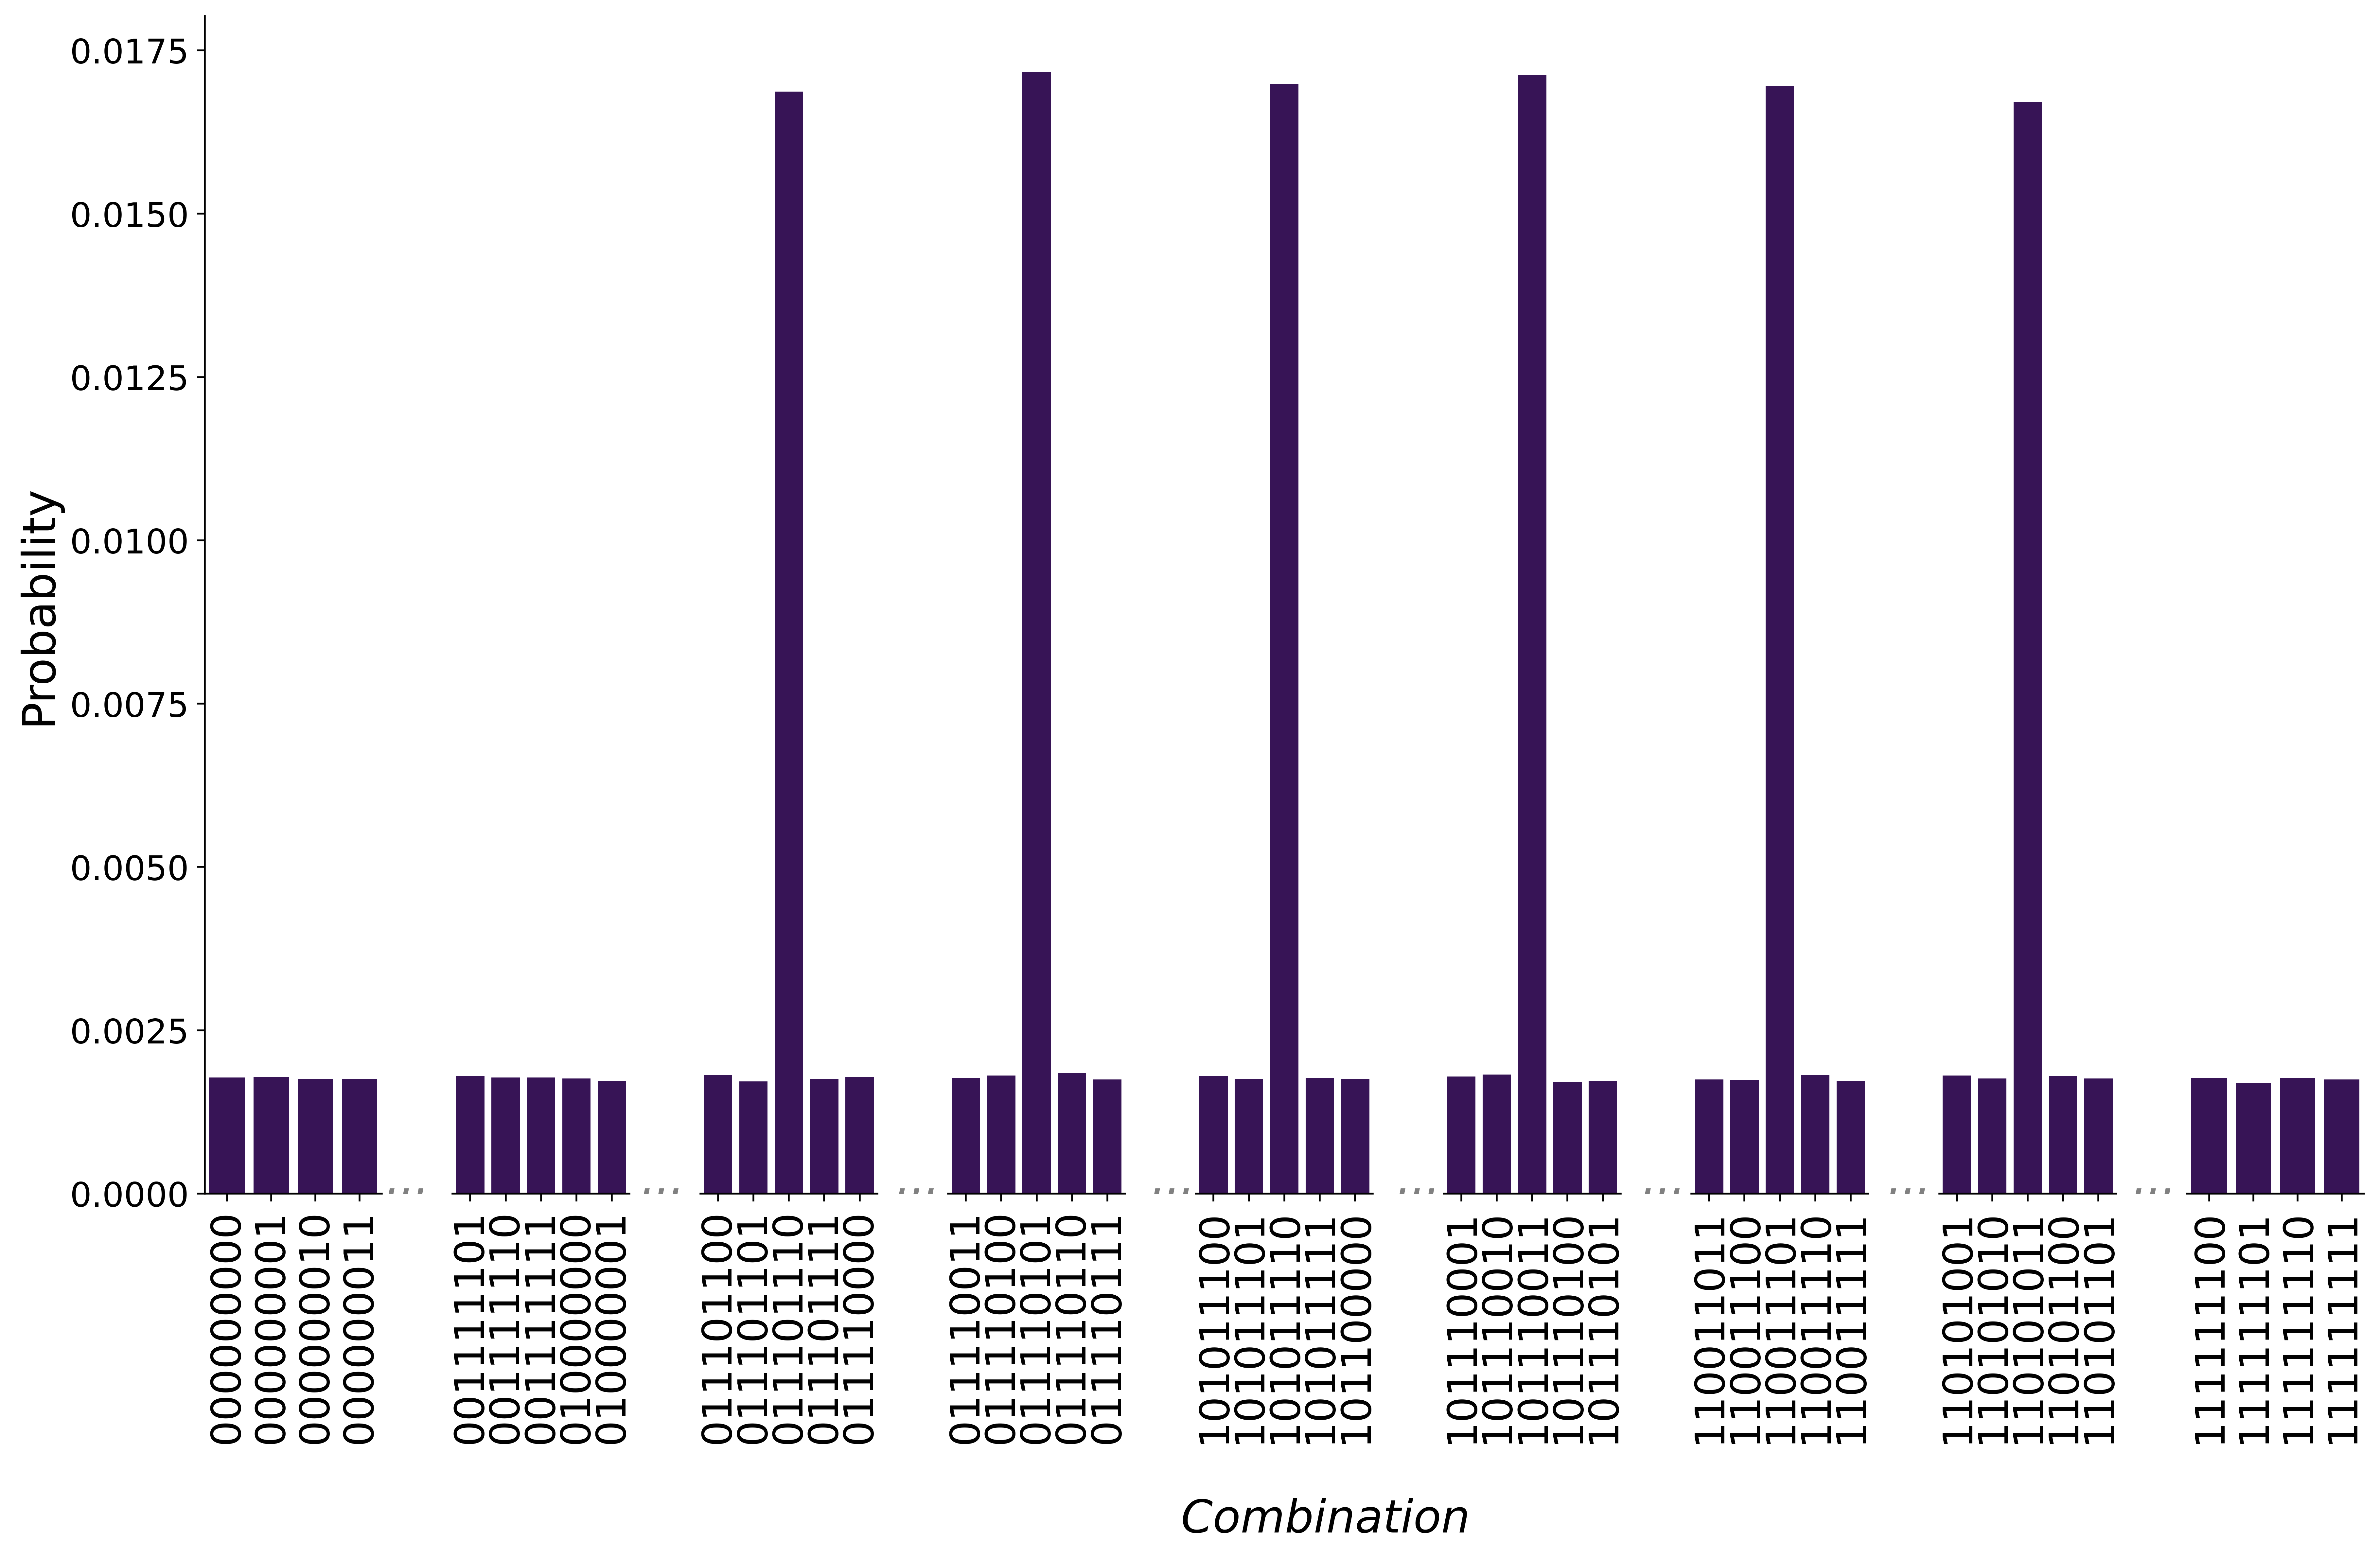
\includegraphics[width=18cm]{Figures/large1iter.png}
\caption{Results from the simulator with one iteration}
\label{After first iteration}
\end{figure}

With performing only one iteration we can see from the plot that correct combinations have probability to be measured circa $0.017$, incorrect less than $0.002$.

\begin{figure}[H]
\centering
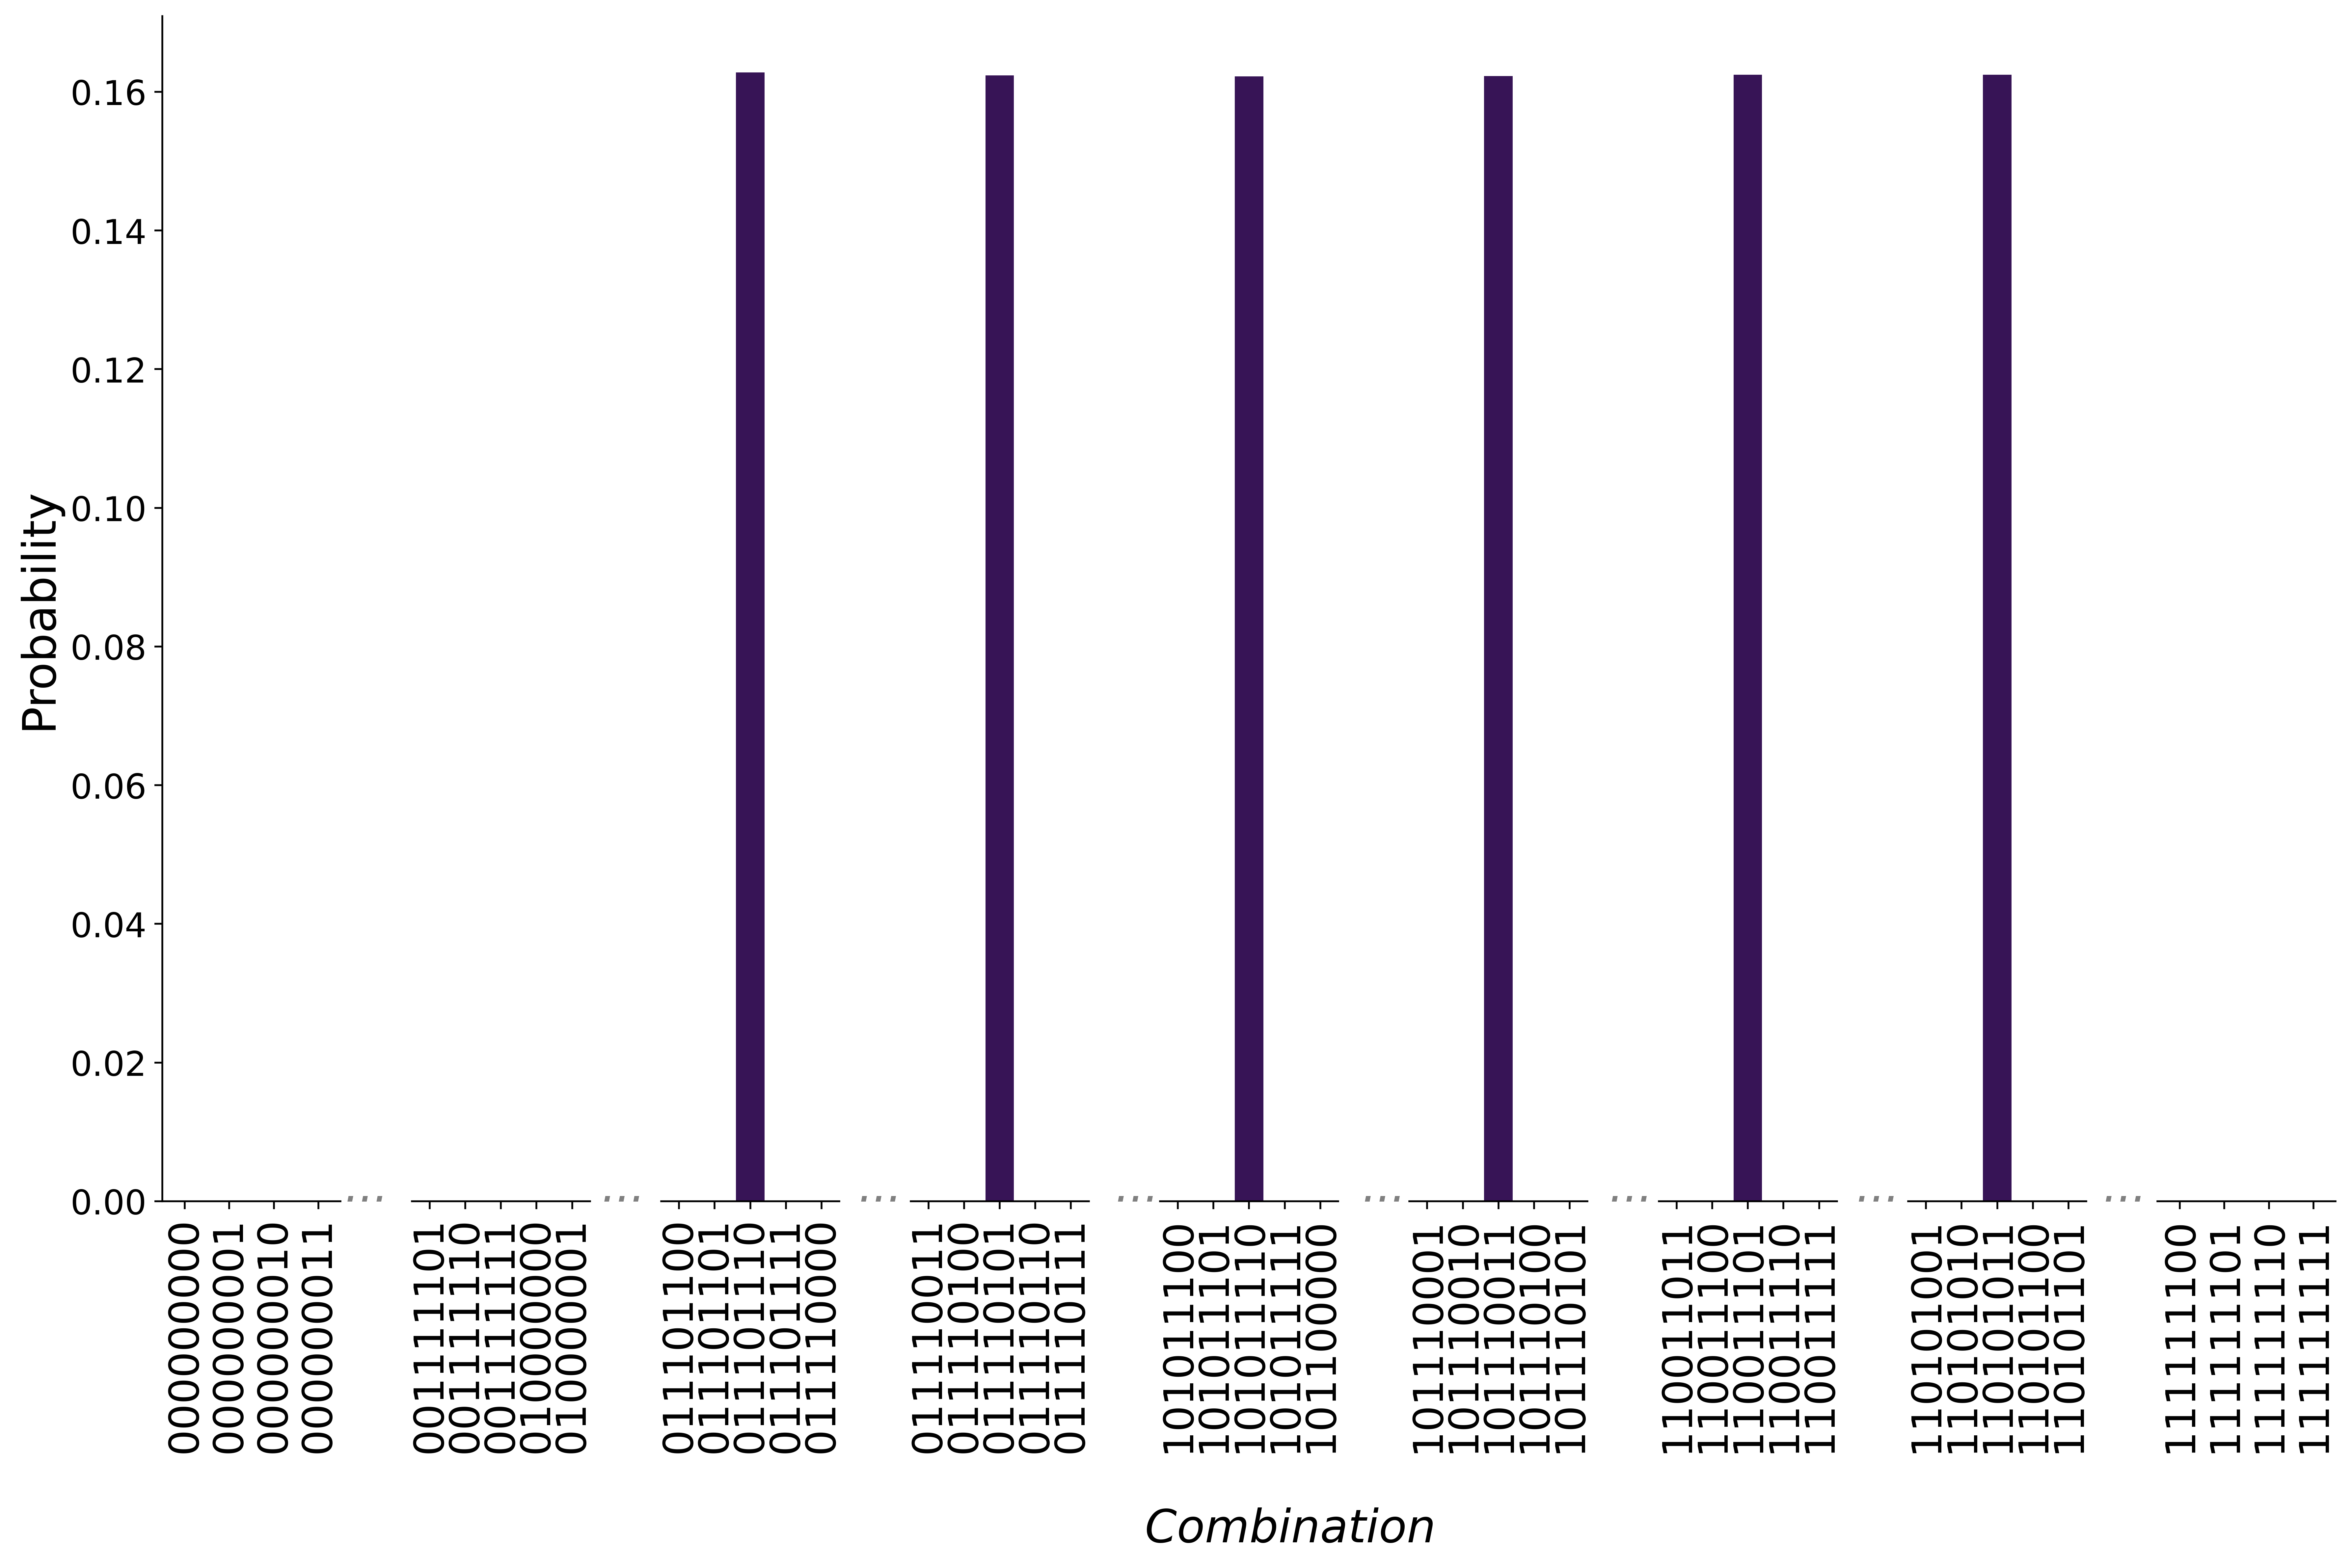
\includegraphics[width=17cm]{Figures/largefinal.png}
\caption{Results from the simulator}
\label{sim_large}
\end{figure}

When we perform optimal number of iterations (in this case, 6 or 7), we get almost ten times improvement with measuring the correct combinations. We also see that there is a very small probability of measuring one of the other $506$ combinations.

It is also important not to confuse that the solution is periodical. With the decimal representation, the results could be interpreted as $\{238, 245, 350, 371, 413, 427\}$. Despite not having any reasonable metric, we can see that intuitively they are distributed unequally.

\chapter{Conclusion}

The goal of the thesis was to define and analyse basics of quantum computing and Grover's algorithm with application to 2 problems.

In chapter \ref{basicschapter} we have defined qubits and the mathematical representation for them, introduced systems of qubits with the introduction of the tensor product for both vectors and matricies. Then we have defined basic quantum gates and controlled gates, which are applied if and only if all the controlling qubits are in state $|1\rangle$, with controlled gates we have demonstrated entanglement, which is crucial for Grover's algorithm. 

In chapter \ref{GA_theo} we have analysed the algorithm. First, we have defined the time complexity and described the motivation for the algorithm with a description of the complexity difference using this algorithm. Then we focused on the inner parts of the algorithm, the oracle, and the diffuser. We derived reccurence equations for the change in qubits' amplitudes with each iteration. We have described a geometrical analysis that consists of reflection and rotation, with the geometrical analysis we derived the optimal number of iterations in eq. \ref{optimal_iter}.

Chapter \ref{Practical_ch} introduced circuits for the Grover's algorithm. We have described how to create an oracle for a problem and described how the circuit works, then we introduced the diffuser and its smaller version with different preparation of the circuit.

The first problem was taken from \cite{qc_grover_ibm}. We have created two quantum circuits to solve it, both were run on the real quantum computer and on simulator. The difference was huge, results from the real quantum computer were flawed, but it was still possible to see the correct results for the problem, on the other hand results from the simulator were flawless and we could simply read the solution to the problem.

The second problem was larger; this meant that the circuit had to be larger. In the first problem we used 5 and 6 qubits in the quantum computer, for the second problem 16 were needed. As we currently don't have access to that big quantum computer our only results were from a simulator, where the results were very good.

Work on this algorithm can be expanded to application on more sophisticated SAT problems or graph problems. It is also possible to focus on making an oracle with fewer gates, so that the decoherence is smaller and the results are better.
%\chapter{Conclusion}

The goal of the thesis was to define and analyse basics of quantum computing and Grover's algorithm with application to 2 problems.

In chapter \ref{basicschapter} we have defined qubits and the mathematical representation for them, introduced systems of qubits with the introduction of the tensor product for both vectors and matricies. Then we have defined basic quantum gates and controlled gates, which are applied if and only if all the controlling qubits are in state $|1\rangle$, with controlled gates we have demonstrated entanglement, which is crucial for Grover's algorithm. 

In chapter \ref{GA_theo} we have analysed the algorithm. First, we have defined the time complexity and described the motivation for the algorithm with a description of the complexity difference using this algorithm. Then we focused on the inner parts of the algorithm, the oracle, and the diffuser. We derived reccurence equations for the change in qubits' amplitudes with each iteration. We have described a geometrical analysis that consists of reflection and rotation, with the geometrical analysis we derived the optimal number of iterations in eq. \ref{optimal_iter}.

Chapter \ref{Practical_ch} introduced circuits for the Grover's algorithm. We have described how to create an oracle for a problem and described how the circuit works, then we introduced the diffuser and its smaller version with different preparation of the circuit.

The first problem was taken from \cite{qc_grover_ibm}. We have created two quantum circuits to solve it, both were run on the real quantum computer and on simulator. The difference was huge, results from the real quantum computer were flawed, but it was still possible to see the correct results for the problem, on the other hand results from the simulator were flawless and we could simply read the solution to the problem.

The second problem was larger; this meant that the circuit had to be larger. In the first problem we used 5 and 6 qubits in the quantum computer, for the second problem 16 were needed. As we currently don't have access to that big quantum computer our only results were from a simulator, where the results were very good.

Work on this algorithm can be expanded to application on more sophisticated SAT problems or graph problems. It is also possible to focus on making an oracle with fewer gates, so that the decoherence is smaller and the results are better.


\printbibliography[heading=bibintoc]

\appendix
%\input{Chapters/Appendix1.tex}
%\input{Chapters/Appendix2.tex}


% Appendix included directly in main LaTeX file. Not all attachments need to be in separate files.
\chapter{Functions with respective solutions to the problems}
\lstinputlisting[label=src:Python code,caption={Functions with respective solutions to the problems}]{SourceCodes/solution_script.py}



\end{document}
